\documentclass[14pt]{article}
\usepackage[utf8]{inputenc}
\usepackage[russian]{babel}
\usepackage[T2A]{fontenc}
\usepackage{vmargin}
\setpapersize{A4}
\setmarginsrb{2cm}{1.5cm}{1cm}{1.5cm}{0pt}{0mm}{0pt}{13mm}
\usepackage{indentfirst}
\usepackage{mathtools}
\usepackage{graphicx}

\begin{document} 

\renewcommand{\vec}[1]{\mbox{\mathversion{bold}$#1$}}
\pagestyle{plain}

\begin{center}
\textbf{
Вопросы к экзамену по теории информации 2022/2023
}
\end{center}

\bigskip
\textbf{1. Формула условной вероятности события.} \\

Для произвольной пары событий \( A, B \subseteq X\) условной вероятностью события \( A \) при условии \( B \) называется величина: \\
\begin{displaymath}
    P(A|B) = \frac{P(AB)}{P(B)};
\end{displaymath}
при \( P(B) \neq 0 \) и величина \( P(A|B) = 0 \) при \( P(B) = 0 \).

\bigskip
\textbf{2. Определение несовместных событий. Определение совместно независимых событий.} \\

События несовместны, если их пересечение - пустое множество. Для несовместных событий вероятность объединения равна сумме
вероятностей событий. Если условие несовместности не выполнено, вероятность объединения становится меньше суммы вероятностей. \\
События \( A, B \subseteq X\) называют независимыми, если: \\
\begin{displaymath}
    P(AB) = P(A)P(B);
\end{displaymath}
Совместно независимыми называют события \( A_1, ..., A_n \subseteq X \) такие, что:
\begin{displaymath}
    P(A_1 ... A_n) = P(A_1)P(A_2) ... P(A_n);
\end{displaymath}

\bigskip
\textbf{3. Формула вероятности совместных события (произведения событий).} \\

\begin{displaymath}
    P(AB) = P(A|B)P(B);
\end{displaymath}

\bigskip
\textbf{4. Формула полной вероятности (апостериорной вероятности).} \\

Формула полной вероятности и формула апостериорной вероятности, или формула Байеса:
\begin{displaymath}
    P(H_j|A) = \frac{P(A|H_j)P(H_j)}{\displaystyle\sum_{m=1}^{M} P(A|H_m)P(H_m)};
\end{displaymath}

\bigskip
\textbf{5. Произведение множеств.} \\

Произведением множеств \( X \) и \( Y \) называется множество: \\
\begin{displaymath}
    Z = XY = \{(x, y) : x \in X, y \in Y\}
\end{displaymath}
множество упорядоченных пар, первый элемент которых принадлежит множеству \( X \), а второй - множеству \( Y \).

\bigskip
\textbf{6. Формула условного распределения вероятностей.} \\

Условным распределением вероятностей на элементах множества \( X \) при фиксированном элементе \( y \in Y \) называется распределение: \\
\begin{displaymath}
p(x|y) = \left\{ \begin{array}{ll}
 \frac{p(x, y)}{p(y)} & \textrm{если \(p(y) \neq 0\),}\\
 0 & \textrm{в противном случае,}\\
  \end{array} \right.
\end{displaymath}
При этом \(x \in X\).

\bigskip
\textbf{7. Условие независимости двух ансамблей.} \\

Ансамбли \(Х\) и \(У\) независимы, если имеют место тождества:
\begin{displaymath}
    x \in X, y \in Y
\end{displaymath}
\begin{displaymath}
    p(x, y) = p(x)p(y)
\end{displaymath}

\bigskip
\textbf{8. Матожидание, дисперсия и корреляционный момент случайных величин.} \\

Математическим ожиданием случайной величины \(x \in X\) называется:
\begin{displaymath}
    \textbf{M}_X[x] = \displaystyle\sum_{x \in X} xp(x)
\end{displaymath}
Другими важными характеристиками случайных величин являются дисперсия: \\
\begin{displaymath}
    \textbf{D}_X[x] = \textbf{M}_X[(x - \textbf{M}_X[x])^2]
\end{displaymath}
и корелляционный момент: \\
\begin{displaymath}
    K_{XY}(x,y) = \textbf{M}_{XY}[(x - \textbf{M}[x])(y - \textbf{M}[y])]
\end{displaymath}
Если для двух случайных величин корреляционный момент равен нулю, случайные величины называют некоррелированными. \\

\bigskip
\textbf{9. Собственная информация сообщения и ее свойства.} \\

Собственной информации \(I(x)\) сообщения x, выбираемого из дискретного ансамбля \(X = \{x, p(x)\}\), называется величина, вычисляемая по формуле: \\
\begin{displaymath}
    I(x) = -\log p(x)
\end{displaymath}
единица измерения - бит. \\

Из определения собственной информации и свойств логарифма непосредственно вытекают следующие свойства собственной информации: \\
\begin{itemize}
    \item Неотрицательность: \(I(x) \geq 0, x \in X\);
    \item Монотонность: если \(x_1, x_2 \in X, p(x_1) \geq p(x_2)\), то \(I(x_1) \leq I(x_2)\);
    \item Аддитивность: для независимых сообщений \( x_1,...,x_n\) имеет место равенство:
    \begin{displaymath}
        I(x_1,...,x_n) = \displaystyle\sum_{i=1}^{n} I(x_i)
    \end{displaymath}
\end{itemize}

\bigskip
\textbf{10. Энтропия дискретного ансамбля.} \\

Энтропией дискретного ансамбля \(X = \{x, p(x)\}\) называется величина: \\
\begin{displaymath}
    H(X) = \textbf{M}[-\log p(x)] = -\displaystyle\sum_{x \in X} p(x)\log p(x)
\end{displaymath}

\bigskip
\textbf{11. Свойство энтропии дискретного ансамбля (свойства 1.3.1-1.3.7).} \\

\begin{itemize}
    \item Свойство 1.3.1: \( H(X) \geq 0\);
    \item Свойство 1.3.2: \( H(X) \leq \log X\). Равенство имеет место в том и только в том случае, когда элементы ансамбля Х равновероятны;
    \item Свойство 1.3.3: Если для двух ансамблей \(X\) и \(Y\) распределения вероятностей представляют собой одинаковые наборы чисел (различающиеся только порядком следования элементов), то \( H(X) = H(Y)\);
    \item Свойство 1.3.4: Если ансамбли \(Y\) и \(Y\) независимы, то \(H(XY) = H(X) + H(Y)\);
    \item Свойство 1.3.5: Энтропия — выпуклая \( \cap \) функция распределения вероятностей на элементах ансамбля \(Х\);
    \item Свойство 1.3.6: Пусть \(X = \{x, p(x)\}\) и \( A \subseteq X\). Введем новый ансамбль \(X' = \{x, p'(x)\}\), задав распределение вероятностей \( p'(x) \) следующим образом: \\
    \begin{displaymath}
    p'(x) = \left\{ \begin{array}{ll}
        \frac{P(A)}{|A|}, & \textrm{\(x \in A\),}\\
        p(x), & \textrm{\(x \notin A\)}\\
    \end{array} \right.
    \end{displaymath}
        Тогда \( H(X') \geq H(X) \) Иными словами, «выравнивание» вероятностей элементов ансамбля приводит к увеличению энтропии;
    \item Свойство 1.3.7: Пусть задан ансамбль \( X \) и на множестве его элементов определена функция  \(g(x)\). Введем ансамбль \( Y = \{y = g(x)\} \). Тогда \( H(X) \leq H(Y)\). Равенство имеет место тогда и только тогда, когда функция \(g(x)\) обратима. 
\end{itemize}

\bigskip
\textbf{12. Энтропия двоичного ансамбля.} \\

Рассмотрим двоичный ансамбль \(X = \{0,1\}\). Положим \(p(1) = p, p(0) = 1 - p = q\). Энтропия этого ансамбля: \\
\begin{displaymath}
    H(X) = -p\log p - q \log q = \eta(p)
\end{displaymath}

Мы ввели специальное обозначение \( \eta(p) \) для энтропии двоичного ансамбля, в котором один из элементов имеет вероятность 2. Эта функция будет часто использоваться. Построим график зависимости \( \eta(p) \) от p при \( p \in [0,1]\). Начнем с крайних точек \(р = 0\) и \(p = 1\). В обоих случаях имеет место неопределенность. Тем не менее, используя правило Лопиталя, легко вычислить предельные значения \(\eta(p)\) при \( p \to 0\) и \( p \to 1\). Получим \(\eta(0) = \eta(1) = 0\). Далее, заметим, что \(\eta(p) = \eta(1 - p)\), то есть функция симметрична относительно оси \( p = frac{1}{2} \). \\

\bigskip
\textbf{13. Условная собственная информация.} \\

Рассмотрим ансамбли \(X=\{x\}\) и \(Y=\{y\}\) и их произведение \(XY = \{(x, y), р(x,y)\}\). \\
Для любого фиксированного \(y \in Y\) можно построить условное распределение вероятностей \( p(x|y)\) на множестве \(X\) и для каждого \( x \in X \) подсчитать собственную информацию: \\
\begin{displaymath}
    I(x|y) = -\log p(x|y)
\end{displaymath}
которую называют условной собственной информацией сообщения \(x\) при фиксированном \(y\).

\bigskip
\textbf{14. Формула условной энтропии при фиксированном событии. Формула условной энтропии ансамбля при фиксированном другом ансамбле.} \\

Энтропия ансамбля \(X\) — средняя информация сообщений \(x \in X\). Усреднив условную информацию \(I(x|y)\) по \(x \in X\), получим величину:
\begin{displaymath}
    H(X|y) = -\displaystyle\sum_{x \in X} p(x|y)\log p(x|y);
\end{displaymath}
называемую условной энтропией \(X\) при фиксированном \(y \in Y\). Заметим, что в определении имеется неопределенность при \( p(x|y) = 0 \).

Вновь введенная энтропия \(H(X|y)\) -- случайная величина, поскольку она зависит от случайной переменной \(y\). Чтобы получить неслучайную информационную характеристику пары вероятностных ансамблей, нужно выполнить усреднение в формуле условной энтропии по всем значениям \(y\), Величина
\begin{displaymath}
    H(X|Y) = -\displaystyle\sum_{x \in X} \displaystyle\sum_{y \in Y} p(x,y) \log p(x,y)
\end{displaymath}
называется условной энтропией ансамбля \(X\) при фиксированном ансамбле \(Y\). \\

\bigskip
\textbf{15. Свойства условной энтропии (свойства 1.4.1-1.4.6).} \\

\begin{itemize}
    \item Свойство 1.4.1: \( H(X|Y) \geq 0 \);
    \item Свойство 1.4.2: \( H(X|Y) \leq H(X) \), причем равенство имеет место в том и только в том случае, когда ансамбли \(X\) и \(Y\) независимы;
    \item Свойство 1.4.3: \( H(XY) = H(X) | H(Y|X) = H(Y) + H(X|Y) \);
    \item Свойство 1.4.4: \( H(X_1...X_n) = H(X_1) + H(X_2|X_1) + H(X_3|X_2X_1) + ... + H(X_n|X_1,...,X_{n-1})\);
    \item Свойство 1.4.5: \( H(X|YZ) \leq H(X|Y) \), причем равенство имеет место в том и только в том случае, когда ансамбли \(X\) и \(Z\) условно независимы при всех \(y \in Y\);
    \item Свойство 1.4.6: \( H(X_1...X_n) \leq \displaystyle\sum_{i=1}^{n} H(X_i) \), причем равенство возможно только в случае совместной независимости ансамблей \(X_1,...,X_{n}\).
\end{itemize}

\bigskip
\textbf{16. Определение стационарного процесса.} \\

Вместо отдельных ансамблей и произведений конечного числа ансамблей мы будем рассматривать теперь — случайные последовательности из произвольного числа событий. Если элементы случайной последовательности - вещественные числа, то такие последовательности называются случайными процессами. 

Процесс называется стационарным, если для любых \(n\) и \(y\) имеет место равенство
\begin{displaymath}
    p(x_1,...,x_n)= p(x_{1+t},...x_{n+t})
\end{displaymath}
в котором подразумевается, что \( x_i = x_{i+t}, i = 1,...,n \).

Случайный процесс стационарен, если вероятность любой последовательности не изменяется при ее сдвиге во времени (не зависит от положения последовательности на оси времени). \\

\bigskip
\textbf{17. Цепь Маркова связности s. Однородная цепь Маркова. Простая цепь Маркова. Матрица
переходных вероятностей цепи Маркова.} \\

Случайный процесс \(x_1, x_2, ...\) называют цепью Маркова связности s, если для любых n и для любых \(\textbf{x} = (x_1,...,x_n) \in X^n\) справедливы соотношения
\begin{displaymath}
    p(x) = p(x_1,...,x_s)p(x_{s+1}|x_1,...,x_s)p(x_{s+2}|x_2,...,x_{s+1}) \times ... \times p(x_n|x_{n-s},...,x_{n-1})
\end{displaymath}

Марковский процесс связности S называется такой процесс, для которого при \( n > s \)
\begin{displaymath}
    p(x_n|x_{1},...,x_{n-1}) = p(x_n|x_{n-s},...,x_{n-1})
\end{displaymath}
то есть условная вероятность текущего значения при известных предшествующих s не зависит от всех других предшествующих значений.

Описание марковского процесса задается начальным распределением вероятностей на последовательностях из первых S значений (состояний) и условными вероятностями вида \(p(x_n|x_{n-s},...,x_{n-1})\) для всевозможных последовательностей \((x_{n-s},...,x_n\). Если указанные условные вероятности не изменяются при сдвиге последовательностей \((x_{n-s},...,x_n\) во времени, марковская цепь называется однородной.

Однородная марковская цепь связности \(s = 1\) называется простой цепью Маркова. Для описания простой цепи Маркова с множеством состояний \(X = \{0,1.....M-1\}\) достаточно указать начальное распределение вероятностей \(\{p(x_1), x_1 \in X\}\) и условные вероятности \\
\begin{displaymath}
    \pi_{ij} = P(x_t = j|x_{t-1} = i), i,j = 0,...,M - 1
\end{displaymath}
называемые переходными вероятностями цепи Маркова.

Переходные вероятности удобно записывать в виде квадратной матрицы размерности \( M \times M \):
\begin{displaymath}
\Pi = 
 \begin{pmatrix}
  \pi_{0,0} & \pi_{0,1} & \cdots & \pi_{0,M-1} \\
  \pi_{1,0} & \pi_{1,1} & \cdots & \pi_{1,M-1} \\
  \vdots  & \vdots  & \ddots & \vdots  \\
  \pi_{M-1,0} & \pi_{M-1,1} & \cdots & \pi_{M-1,M-1} \\
 \end{pmatrix}
\end{displaymath}
называемой матрицей переходных вероятностей.

\bigskip
\textbf{18. Стационарное распределение для цепи Маркова. Эргодические цепи. Понятие состояния
цепи. Неприводимые цепи.} \\

Пусть существует стохастический вектор \textbf{p} \\
\begin{displaymath}
    \textbf{p} = \textbf{p}\Pi
\end{displaymath}
Стохастический вектор \textbf{p}, удовлетворяющий уравнению выше, называется стационарным распределением для цепи Маркова, задаваемой матрицей переходных вероятностей \(\Pi\).

Финальным распределением вероятностей называют вектор
\begin{displaymath}
    \textbf{\(p_{\infty}\)} = \lim\limits_{t \to \infty} \textbf{$p_t$} = \lim\limits_{t \to \infty} \textbf{$p_1$} \Pi^t
\end{displaymath}
(если указанный предел существует).

Для широкого класса простых цепей Маркова предел финального распределения не зависит от начального распределения \(p_1\) и равен единственному решению уравнения \(\textbf{p} = \textbf{p}\Pi\), то есть \(p_{\infty} = p\). Такие цепи называют эргодическими.

Множество состояний С называется замкнутым, если никакое состояние вне С не может быть достигнуто из состояния, входящего в С. Цепь называется неприводимой, если в ней содержится не больше одного замкнутого множества. Цепь Маркова неприводима, в частности, тогда, когда все ее состояния достижимы друг из друга.

\bigskip
\textbf{19. Энтропия на букву последовательности.} \\

Для стационарного процесса энтропия распределения вероятностей на таких блоках \( H(X_1...X_n) = H(X^n)\) не зависит от расположения блока во времени, ее называют n-мерной энтропией источника.

Величина \(H(X^n)\) определяет среднее количество информации в последовательности из n букв. Нормированную величину
\begin{displaymath}
    H_n(X) = \frac{H(X^n)}{n}
\end{displaymath}
называют энтропией на букву последовательности длины n.

\bigskip
\textbf{20. Свойства двух информационных мер (теорема 1.5: положения A-D).} \\

\textbf{ТЕОРЕМА 1.5.} Для дискретного стационарного источника:
\begin{itemize}
    \item A. \(H(X|X^n)\) не возрастает с увеличением n;
    \item B. \(H_n(X)\) не возрастает с увеличением n;
    \item C. \(H_n(X) \geq H(X|X^{n-1})\);
    \item D. \( \lim\limits_{n \to \infty} H_n(X) = \lim\limits_{n \to \infty} H(X|X^n)\);
\end{itemize}

\bigskip
\textbf{21. Энтропия на сообщение дискретного постоянного источника.} \\

В качестве дискретного постоянного источника рассматривается дискретный стационарный источник без памяти. По свойствам энтропии для источника без памяти имеем: \\
\begin{displaymath}
    H(X_1...X_n) = H(X_1)+...+H(X_n)
\end{displaymath}
\begin{displaymath}
    H(X^n) = nH(X)
\end{displaymath}
Поделив обе стороны тождества на \(n\), получим, что при всех \(n\) справедливо равенство:
\begin{displaymath}
    H_n(X) = H(X)
\end{displaymath}
И, следовательно,
\begin{displaymath}
    H_{\infty}(X) = H(X)
\end{displaymath}
Энтропия на сообщение дискретного постоянного источника в точности равна его одномерной энтропии.

\bigskip
\textbf{22. Энтропия на сообщение Марковского источника.} \\

Энтропия на сообщение марковского источника. Для стационарного источника, описываемого моделью цепи Маркова связности S, можем записать: \\
\begin{displaymath}
    H(X|X^n) = H(X_{n+1}|X_1,...,X_n) = H(X_{n+1}|X_{n-s+1},...,X_n) = H(X|X^s)
\end{displaymath}
Правая часть не зависит от n, значит, \\
\begin{displaymath}
    H(X|X^{\infty}) = H(X|X^s)
\end{displaymath}
Используя стационарность и свойства условной энтропии, запишем: \\
\begin{displaymath}
    H(X^n) = H(X_1...X_sX_{s+1}...X_n) = H(X_1...X_s) + H(X_{s+1}...X_n|X_1,...,X_s)
\end{displaymath}
Из \\
\begin{displaymath}
    H(X_{s+1}...X_n|X_1,...,X_s) = H(X_{s+1}|X_1,...,X_s) + H(X_{s+2}|X_1,...,X_{s+1}) + ... + H(X_n|X_1,...,X_{n-1})
\end{displaymath}
учитывая марковость и стационарность, получаем: \\
\begin{displaymath}
    H(X_{s+1}...X_n|X_1,...,X_s) = (n - s)H(X|X^s)
\end{displaymath}
Теперь можно поделить обе части на \(n\) и устремить \(n\) к бесконечности: \\
\begin{displaymath}
    H_{\infty}(X) = H(X|X^s)
\end{displaymath}
Перепишем выражение с \((n - s)H(X|X^s)\) в виде: \\
\begin{displaymath}
    H_n(X) = H(X|X^s) + \frac{s}{n}(H_s(X) - H(X|X^s)) = H(X|X^n) + \frac{s}{n}(H_s(X) - H(X|X^s)) 
\end{displaymath}
Отсюда видна разница между \(H_n(X)\) и \(H(X|X^n)\).

\bigskip
\textbf{23. Определение равномерного кода. Мощность кода. Скоростью равномерного кода.} \\

Равномерным кодом длины \(n\) называется любое подмножество \(C\) множества \(A^n\) то есть любое подмножество множества последовательностей длины \(n\). Элементы кода \(C\) называют кодовыми словами. Мощность кода \(|C|\) - это количество кодовых слов в коде \(C\).

Скоростью равномерного кода называется величина: \\
\begin{displaymath}
    R = \frac{\lceil \log |C| \rceil}{N}
\end{displaymath}
(бит / букву источника), где \(\lceil a \rceil\) обозначает округление числа \(a\) вверх до ближайшего целого.

\bigskip
\textbf{24. Условие взаимно однозначного кодирования.} \\

Работа кодера (алгоритм кодирования) описывается отображением множества \(X^N\) на множество слов кода \(C\). Декодирование задается отображением \(C\) на \(X^N\).

Если оба отображения взаимно однозначные, то на выходе декодера можно будет получить точную копию передаваемой последовательности.

Взаимно однозначное кодирование возможно только тогда, когда: \\
\begin{displaymath}
    |X|^N \leq |C|
\end{displaymath}
или
\begin{displaymath}
    R \geq \log |X| \geq H(X)
\end{displaymath}

Если буквы источника не равновероятны (\(H(X) < \log |X|\)), то скорость кода окажется заведомо больше энтропии источника.

\bigskip
\textbf{25. Неравенство Чебышева для суммы независимых случайных величин.} \\

Рассмотрим дискретную случайную величину \(X = \{x, p(x)\}\). Предположим, что все ее значения \(x \in X\) неотрицательны, и при этом предположении оценим вероятность события \(P(x \geq a)\) для некоторого числа \(A > 0\).
\begin{displaymath}
    P(x \geq a) = \sum_{x \geq A} p(x) \leq \sum_{x \geq A} \frac{x}{A}p(x) \leq \frac{1}{A}\sum_{x \geq A} xp(x) = \frac{\textbf{M}[x]}{A}
\end{displaymath}

Введем обозначение \(m_x = \textbf{M}[x]\). Тогда \\
\begin{displaymath}
    P(x \geq a) \leq \frac{m_x}{A}
\end{displaymath}

Для оценки искомой вероятности достаточно знать только ее математическое ожидание.

Пусть \(X = \{x, p(x)\}\) - произвольная (необязательно неотрицательная) случайная величина. Для произвольного \( \epsilon > 0 \) оценим вероятность \( P|x - m_x| \geq \epsilon \). \\

Положим \(y = |x - m_x|\). Для этой неотрицательной случайной величины получаем
\begin{displaymath}
    P(y \geq \epsilon) = P(y^2 \geq \epsilon^2) \leq \frac{\textbf{M}[y^2]}{\epsilon^2} = \frac{\textbf{M}[(x - m_x)^2]}{\epsilon^2} = \frac{\textbf{D}[x]}{\epsilon^2}
\end{displaymath}

Результат запишем в виде: \\
\begin{displaymath}
    P(|x - m_x| \geq \epsilon) \leq \frac{\sigma_x^2}{\epsilon^2}
\end{displaymath}
где \(\sigma_x^2 = \textbf{D}[x]\). Данное неравенство называется неравенством Чебышева.

Рассмотрим теперь последовательность из \(n\) независимых случайных величин \(X_i, i = 1,\ldots,n,\) имеющих одинаковое математическое ожидание \(m_x\) и одинаковую дисперсию \(\sigma_x^2\). Найдем \\
\begin{displaymath}
    P(|\frac{1}{n}\sum_{i=1}^{n} x_i - m_x| \geq \epsilon)
\end{displaymath}

Положим \\
\begin{displaymath}
    y = \frac{1}{n}\sum_{i=1}^{n} x_i
\end{displaymath}

Учитывая независимость случайных величин \(x_1,\ldots,x_n\), получим \\
\begin{displaymath}
    \textbf{M}[y] = m_x
\end{displaymath}
\begin{displaymath}
    \textbf{D}[y] = \frac{1}{n}\sigma_x^2
\end{displaymath}

Применив к случайным величинам \(y\) неравенство Чебышева \\
\begin{displaymath}
    P(|\frac{1}{n}\sum_{i=1}^{n} x_i - m_x| \geq \epsilon) \leq \frac{\sigma_x^2}{n\epsilon^2}
\end{displaymath}
неравенство Чебышева для суммы независимых случайных величин.

\bigskip
\textbf{26. Прямая теорема кодирования (теорема 1.6 с доказательством).} \\

\textbf{ТЕОРЕМА 1.6.} Пусть \(H\) - энтропия дискретного постоянного источника. Для любых \(\epsilon,\delta > 0\) существует \(n_0\) такое, что для любого \(n > n_0\) найдется равномерный код, кодирующий источник блоками длиной \(n\) со скоростью \( R \leq H + \delta\) и вероятностью ошибки \(P_e \leq \epsilon\).

\textbf{Доказательство.} Правило кодирования полностью описывается выбором множества \(T \subseteq X^n\) однозначно кодируемых последовательностей сообщений источника.

Выберем \(T \subseteq X^n\) следующим образом:
\begin{displaymath}
    T = \Big\{x: |\frac{1}{n}I(x) - H| \leq \delta_0\Big\}   (1.20)
\end{displaymath}
где через \(I(x) = -\log p(x)\) обозначена собственная информация последовательности \(\textbf{x} \in X^n\), а через \(\delta_0\) обозначена положительная константа, значение которой будет выбрано позже.

Множество \(T\) состоит из таких последовательностей, средняя собственная информация которых весьма близка к энтропии, если величина \(\delta_0\) достаточно мала.

Множество \(T\) называется множеством типичных последовательностей. Это множество играет важную роль в теории информации.

Из (1.20) следует, что вероятности последовательностей множества \(T\) удовлетворяют неравенствам
\begin{displaymath}
    2^{-n(H+\delta_0)} \leq p(x) \leq 2^{-n(H-\delta_0)}
\end{displaymath}

Левая и правая части могут рассматриваться как оценки снизу и сверху для вероятностей последовательностей из \(T\). Для оценки числа элементов в этом множестве заметим, что
\begin{displaymath}
    1 \geq P(T) = \sum_{x \in T} p(x) \geq |T| \min_{x \in T} p(x) \geq |T| 2^{-n(H+\delta_0)}
\end{displaymath}

Следовательно
\begin{displaymath}
    |T| \leq 2^{n(H+\delta_0)}
\end{displaymath}

По определению скорость кода: 
\begin{displaymath}
    R = \frac{\lceil \log |T| \rceil}{n} \leq H + \delta_0 + \frac{1}{n}      (1.23)
\end{displaymath}

Ошибка кодирования имеет место тогда, когда источник порождает последовательность, не входящую в множество \(T\). Поэтому вероятность ошибки \(P_e\) удовлетворяет соотношениям:
\begin{displaymath}
    P_e = P(\textbf{x} \notin T) = P\Big(\Big|\frac{1}{n}I(x) - H \Big| > \delta_0 \Big) = P\Big(\Big|\frac{1}{n}\sum_{i=1}^{n}I(x_i) - H \Big| > \delta_0 \Big)      (1.24)
\end{displaymath}

Последний переход учитывает, что буквы источника независимы и, в силу аддитивности собственной информации, информация последовательности равна сумме информации отдельных букв
\begin{displaymath}
    \textbf{M}[I(x)] = H
\end{displaymath}

К выражению (1.24) можно применить неравенство Чебышева:
\begin{displaymath}
    P_e \leq \frac{\textbf{D}[I(x)]}{n\delta_0^2}    (1.25)
\end{displaymath}

Значит, для любой наперед заданной величины \(\delta_0\) можно теперь подобрать длину кодируемых блоков \(n\) так, чтобы вероятность ошибки была меньше любого \(\epsilon\).

Положим теперь \(\delta_0 = \frac{\delta}{2}\). При \(n \geq n_{01} = \frac{\textbf{D}[I(x)]}{\delta^2 \epsilon}\) из (1.25) имеем \(P_e \leq \epsilon\).

Из (1.23) следует, что при \(n \geq n_{02} = \frac{2}{\delta}\) выполняется условие \(R < H + \delta\). Следовательно, при \(n \leq n_0 = max(n_{01}, n_{02})\) скорость кода \(R\) и вероятность ошибки \(P_e\) удовлетворяют требованиям теоремы.

\bigskip
\textbf{27. Обратная теорема кодирования (теорема 1.7 с доказательством).} \\

\textbf{ТЕОРЕМА 1.7.} Для дискретного постоянного источника с энтропией \(H\) существует \(\epsilon > 0\) такое, что для любого \(\delta > 0\) для любого равномерного кода со скоростью \(R \leq H - \delta\) вероятность ошибки удовлетворяет неравенству \(P_e \geq \epsilon\).

\textbf{Доказательство} [от обратного] Если представить, что сколь угодно точное кодирование возможно при скорости меньшей, чем энтропия источника. То необходимо для заданного источника указать некоторую строго положительную независящую от длины кодируемых последовательностей величину \( \epsilon \), которая была бы оценкой снизу вероятности ошибки любого кода со скоростью \( R \leq H - \delta\).

Код полностью описывается выбором множества \(T_1\) однозначно кодируемых последовательностей. По определению, скорость кода равна \(R = \lceil \log |T_1| \rceil / n\), следовательно, код содержит
\begin{displaymath}
    |T_1| \leq 2^{nR} \leq 2^{n(H-\delta)}
\end{displaymath}
кодовых слов. Вместо вычисления нижней оценки для вероятности ошибки \(P_e\) построим оценку сверху для вероятности правильного кодирования
\begin{displaymath}
    P_c = 1 - P_e = \sum_{x \in T_1} p(x)    (1.27)
\end{displaymath}

Введем вспомогательное множество:
\begin{displaymath}
    T = \Big\{x: |\frac{1}{n}I(x) - H| \leq \delta_0\Big\}
\end{displaymath}
где через \(I(x) = -\log p(x)\) обозначена собственная информация последовательности \(\textbf{x} \in X^n\), а через \(\delta_0\) обозначена положительная константа.

Разобьем сумму в правой части (1.27) на две части:
\begin{displaymath}
    P_c = \sum_{x \in T_1 \cap T} p(x) + \sum_{x \in T_1 \cap T^c} p(x)
\end{displaymath}
где через \(T^c\) обозначено дополнение к множеству \(T\).

Оценим вторую сумму следующим образом:
\begin{displaymath}
    \sum_{x \in T_1 \cap T^c} p(x) \leq \sum_{x \in T^c} p(x) = P(T^c) = P(x \notin T)
\end{displaymath}

С помощью неравенства Чебышева получаем оценку:
\begin{displaymath}
    \sum_{x \in T_1 \cap T^c} p(x) \leq \frac{\textbf{D}[I(x)]}{n\delta_0^2}
\end{displaymath}

Для первой из двух сумм:
\begin{displaymath}
    \sum_{x \in T_1 \cap T} p(x) \leq |T_1 \cap T| \max_{x \in T_1 \cap T} p(x) \leq |T_1| \max_{x \in T_1 \cap T} p(x) \leq |T_1| \max_{x \in T} p(x)     (1.31)
\end{displaymath}

Здесь мы сначала оценили сумму сверху, умножив число слагаемых на максимальное слагаемое. Затем использовали неравенство \(|T_1 \cap T| \leq |T_1|\). Последний переход основан на том, что при расширении области поиска максимума максимальное значение не уменьшается.

Подставим в (1.31) оценку мощности кода и оценку максимальной вероятности последовательностей из \(T\):
\begin{displaymath}
    \sum_{x \in T_1 \cap T} p(x) \leq 2^{n(H-\delta)}2^{-n(H-\delta_0)} = 2^{-n(\delta-\delta_0)}
\end{displaymath}

Подстановка приводит к следующей оценке сверху для вероятности правильного кодирования:
\begin{displaymath}
    P_c \leq 2^{-n(\delta-\delta_0)} + \frac{\textbf{D}[I(x)]}{n\delta_0^2}   (1.33)
\end{displaymath}

Пусть \(\delta\) - произвольное положительное число. Выберем теперь значение параметра \(\delta_0\) равным \(\delta_0 = \delta / 2\). При таком выборе правая часть неравенства (1.33) убывает с увеличением \(n\).

Поскольку мы убедились, что с увеличением длины кодируемых блоков вероятность ошибки не только не убывает, но и стремится к 1, то для того чтобы окончательно доказать теорему, нужно установить, что и при конечных длинах блоков вероятность ошибки остается
большой.

Вероятность ошибки положительна при любых длинах блоков \(n\). Поскольку мы договорились о том, что все буквы источника имеют положительные вероятности, для достижения нулевой вероятности ошибки нужно назначить кодовое слово каждой последовательности сообщений, то есть объем кода должен удовлетворять неравенству
\begin{displaymath}
    |T_1| \geq |X|^n
\end{displaymath}

Для этого скорость кода должна быть
\begin{displaymath}
    R \geq \log |T_1|/n \geq \log |X|    (1.34)
\end{displaymath}

Из свойства 1.3.2 следует, что \(H(X) \leq \log |X|\) и, значит, (1.34) входит в противоречие с условиями теоремы, поскольку скорость должна быть меньше энтропии.

Вероятность ошибки положительна при любых \(n\).

Обозначим через \(n_0\) такое значение длины последовательностей \(n\), что при \(n \geq n_0\) справедливо неравенство \(P_c \leq 1/2\). При этом, конечно, вероятность ошибки \(P_e \geq 1/2\). Теперь обозначим через \( \epsilon_0\) минимальную вероятность ошибочного кодирования по всем \(n = 1,2,\ldots,n_0 - 1\).

Поскольку \(\epsilon_0 > 0\), то примем \(\epsilon = min\{\epsilon_0, 1/2\}\). Тогда получаем, что неравенство \(P_e \geq \epsilon\), справедливое при всех \(n = 1,2,\ldots\).

Таким образом, мы определили независящую от длины кода \(n\) нижнюю границу вероятности ошибки \(\epsilon\) для всех кодов со скоростью \(R \leq H - \delta\).

\bigskip
\textbf{28. Источник с памятью (теорема 1.8 с доказательством).} \\

\textbf{ТЕОРЕМА 1.8.} Для любого \(\delta > 0\) имеют место следующие утверждения:
\begin{itemize}
    \item \(\lim\limits_{n \to \infty} P(T_n(\delta)) = 1\)
    \item Для любого натурального \(n\) справедливо неравенство:
        \begin{displaymath}
            |T_n(\delta)| \leq 2^{n(H(X) + \delta)}
        \end{displaymath}
    \item Для любого \(\epsilon > 0\) существует \(n_0\) такое, что при всех \(n \geq n_0\):
        \begin{displaymath}
            |T_n(\delta)| \geq (1 - \epsilon)2^{n(H(X) - \delta)}
        \end{displaymath}
    \item Для \(x \in T_n(\delta)\):
        \begin{displaymath}
            2^{-n(H(X) + \delta)} \leq p(x) \leq 2^{-n(H(X) - \delta)}
        \end{displaymath}
\end{itemize}

\textbf{Доказательство.} Первое утверждение следует из (1.29) и (1.30). Второе совпадает с (1.27), четвертое - с (1.26). Остановимся на третьем утверждении.

Из первого утверждения следует, что для любого \(\epsilon > 0\) найдется \(n_0\) такое, что при \(n > n_0\) имеет место неравенство
\begin{displaymath}
    P(T_n(\delta)) \geq 1 - \epsilon (1.36)
\end{displaymath}

Оценивая вероятность \(T_n(\delta)\) как произведение числа элементов в множестве на величину максимального элемента и применяя утверждение 4, получаем
\begin{displaymath}
    P(T_n(\delta)) \leq |T_n(\delta)| \max_{x \in T_n(\delta)} p(x) \leq |T_n(\delta)|2^{-n(H(X)-\delta)} (1.37)
\end{displaymath}

Из (1.36) и (1.37) следует утверждение 3

\bigskip
\textbf{29. Неравномерное кодирование. Понятие префиксного кода. Описание двоичного кодового дерева. Средняя длина кодовых слов.} \\

Для некоторого дискретного источника \(X\) с известным распределением вероятностей \(\{p(x), x \in X\}\) требуется построить эффективный неравномерный двоичный код над алфавитом \(A = \{a\}\). Рассмотрим кодирование в двоичных символах \(A = \{0,1\}\).

Неравномерный побуквенный код \(C = \{c\}\) объемом \(|C| = M\) над алфавитом \(A\) определяется как произвольное множество последовательностей одинаковой или различной длины из букв алфавита \(A\).

Код является однозначно декодируемым, если любая последовательность символов из \(A\) единственным способом разбивается на отдельные кодовые слова.

Если ни одно кодовое слово не является началом другого, код называется префиксным. Префиксные коды являются однозначно декодируемыми. Префиксность - достаточное, но не необходимое условие для однозначной декодируемости.

\begin{figure}[ht!]
\centering
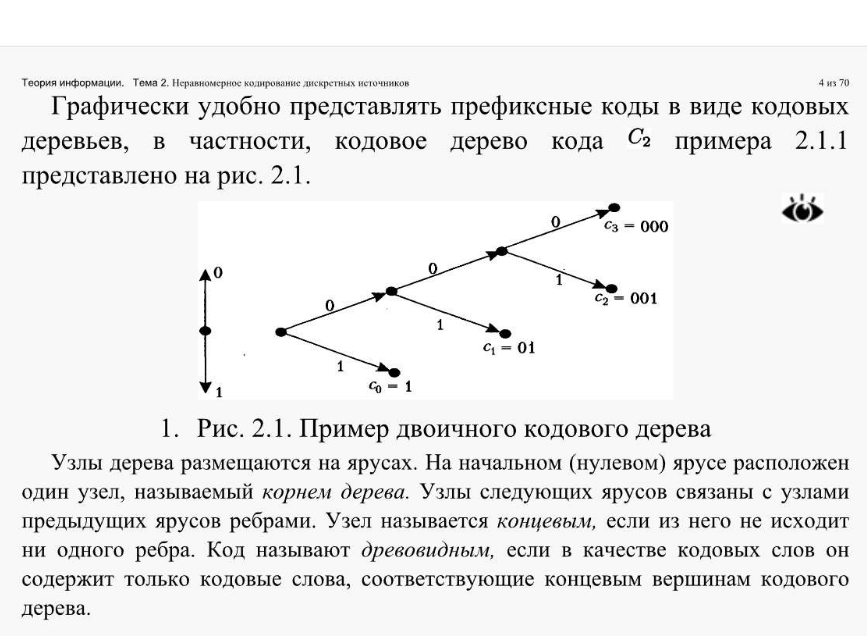
\includegraphics[width=90mm]{code_tree.png}
\caption{Описание двоичного кодового дерева}
\end{figure}

Рассмотрим источник \(X = \{1,\ldots,M\}\), который порождает буквы с вероятностями \(\{p_1,\ldots,p_M\}\). Пусть для кодирования букв источника выбран код \(C = \{c_1,\ldots,c_M\}\) с длинами кодовых слов \(l_1,\ldots,l_M\) соответственно.

Средней длиной кодовых слов называется величина:
\begin{displaymath}
    \bar{l} = \textbf{M}[l_i] = \sum_{i=1}^{M} p_i l_i
\end{displaymath}

\bigskip
\textbf{30. Неравенство Крафта.} \\

\textbf{ТЕОРЕМА 2.1.} Необходимым и достаточным условием существования префиксного кода объемом \(M\) с длинами кодовых слов \(l_1,\ldots,l_M\) является выполнение неравенства Крафта:
\begin{displaymath}
    \sum_{i=1}^{M} 2^{-l_i} \leq 1
\end{displaymath}

\bigskip
\textbf{31. Условие существования префиксного кода (теорема 2.1 с доказательством).} \\

\textbf{ТЕОРЕМА 2.1.} Необходимым и достаточным условием существования префиксного кода объемом \(M\) с длинами кодовых слов \(l_1,\ldots,l_M\) является выполнение неравенства Крафта:
\begin{displaymath}
    \sum_{i=1}^{M} 2^{-l_i} \leq 1
\end{displaymath}

\textbf{Доказательство.} Начнем с необходимости.

Рассмотрим двоичное кодовое дерево произвольного префиксного кода объемом \(M\) с длинами кодовых слов \(l_1,\ldots,l_M\). Выберем целое число \(L\) такое, что \(L \geq max_i l_i\). Проложим все пути в дереве до яруса с номером \(L\). На последнем ярусе мы получим \(2^L\) вершин.

Концевая вершина искомого кодового дерева, расположенная на глубине \(l_i\), имеет два потомка на глубине \(l_i + 1\), 4 потомка на глубине \(l_i + 2\) и т.д. На глубине \(L\) будет \(2^{L-l_i}\) потомков этой вершины.

Множество потомков различных кольцевых вершин не пересекаются, поэтому суммарное число потомков не превышает общего числа вершин на ярусе \(L\). Получаем неравенство:
\begin{displaymath}
    \sum_{i=1}^{M} 2^{L-l_i} \leq 2^L
\end{displaymath}

Поделив обе части на \(2^L\), получим требуемый результат.

Чтобы убедиться в достаточности, нужно показать, что из справедливости (2.1) вытекает существование кода с заданным набором длин кодовых слов. Будем считать \(l_i\) упорядоченными по возрастанию.

Из общего числа \(2^{l_1}\) вершин на ярусе \(l_1\) выберем одну любую вершину, сделаем ее концевой и закрепим ее за первым кодовым словом. Продолжим оставшиеся вершины до радиуса \(l_2\). Из общего числа возможных вершин нужно исключить \(2^{l_2-l_1}\) вершин, которые принадлежат поддереву, начинающемуся в узле, соответствующем первому слову. На ярусе \(l_2\) останется
\begin{displaymath}
    2^{l_2} - 2^{l_2-l_1} \geq 1
\end{displaymath}
вершин. Поделим обе его части на \(2^{l_2}\). Сделаем одну из этих вершин концевой и закрепим ее за вторым словом. Аналогично, для третьего слова мы получим множество из
\begin{displaymath}
    2^{l_3} - 2^{l_3-l_2} - 2^{l_3-l_1} \geq 1
\end{displaymath}

В силу (2.1) всегда найдется одна для третьего слова. Продолжая построение, на последнем ярусе с номером \(M\) получаем
\begin{displaymath}
    2^{l_M} - 2^{l_M-l_{M-1}} - 2^{l_M-l_{M-2}} - \ldots -  2^{l_M-l_{1}}
\end{displaymath}
вершин. Это число не меньше 1, если неравенство (2.1) верно.

\bigskip
\textbf{32. Условие существования однозначно декодируемого двоичного кода (теорема 2.2 с доказательством).} \\

\textbf{ТЕОРЕМА 2.2.} Для любого однозначно декодируемого двоичного кода объемом \(M\) с длинами кодовых слов \(l_1,\ldots,l_M\) справедливо неравенство
\begin{displaymath}
    \sum_{i=1}^{M} 2^{-l_i} \leq 1
\end{displaymath}

\textbf{Доказательство.} Без потери общности можно считать \(l_M\) наибольшей из длин кодовых слов. Выберем некоторое натуральное число \(N\) и запишем \(N\)-ю степень левой части неравенства в виде
\begin{displaymath}
    \Big(\sum_{i=1}^{M} 2^{-l_i} \Big)^N = \underbrace{\Big(\sum_{i_1=1}^{M} 2^{-l_{i_1}} \Big) \ldots \Big(\sum_{i_N=1}^{M} 2^{-l_{i_N}} \Big)}_{N сомножителей} = \sum_{i_1=1}^{M} \ldots \sum_{i_N=1}^{M} 2^{-(l_{i_1}+\ldots+l_{i_N})}
\end{displaymath}

В правой части имеем \(M^N\) слагаемых. Их мы перегруппируем, упорядочив по величине суммы длин кодовых слов \(l_{i_1}+\ldots+l_{i_N}\). Обозначим через \(A_L\) количество таких последовательностей кодовых слов, сумма длин которых равна \(l_{i_1}+\ldots+l_{i_N} = L\). Тогда
\begin{displaymath}
    \Big(\sum_{i=1}^{M} 2^{-l_i} \Big)^N = \sum_{L=1}^{Nl_M} A_L 2^{-L}
\end{displaymath}

\(A_L\), то есть число таких последовательностей из \(N\) кодовых слов, суммарная длина которых в точности равна \(L\), не может быть больше общего числа двоичных последовательностей длиной \(L\). Таким образом, \(A_L \leq 2^L\). Поэтому
\begin{displaymath}
    \Big(\sum_{i=1}^{M} 2^{-l_i} \Big)^N \leq \sum_{L=1}^{Nl_M} 2^L 2^{-L} = Nl_M
\end{displaymath}

Извлечем из обеих частей корень \(N\)-й степени. Получим
\begin{displaymath}
    \sum_{i=1}^{M} 2^{-l_i} \leq (Nl_M)^{1/N} = 2^{\frac{\log (Nl_M)}{N}}
\end{displaymath}

Неравенство справедливо при любых \(N\). Перейдя к пределу при \(N \to \infty\), в правой части получим 1, что и доказывает теорему.

\bigskip
\textbf{33. Прямая теорема побуквенного неравномерного кодирования (теорема 2.3 с доказательством).} \\

\textbf{ТЕОРЕМА 2.3.} Для ансамбля \(X = \{x,p(x)\}\) с энтропией \(H\) существует побуквенный неравномерный префиксный код со средней длиной кодовых слов \(\bar{l} < H + 1\).

\textbf{Доказательство.} Рассмотрим источник над алфавитом \(Х = \{1,...,M\}\) с вероятностями букв \(p_1,\ldots,p_M\). Сопоставим букве \(x_m\) кодовое слово длиной \(l_m = \lceil -\log p_m \rceil\) при \(m =\{1,...,M\}\).

Префиксный код с таким набором длин кодовых слов в соответствии с теоремой 2.1 существует, поскольку длины кодовых слов удовлетворяют неравенству Крафта:
\begin{displaymath}
    \sum_{m=1}^{M} 2^{-l_m} = \sum_{m=1}^{M} 2^{-\lceil -\log p_m \rceil} \leq \sum_{m=1}^{M} 2^{\log p_m} = \sum_{m=1}^{M} p_m = 1
\end{displaymath}

Средняя длина кодовых слов кода
\begin{displaymath}
    \bar{l} = \sum_{m=1}^{M} p_m l_m = \sum_{m=1}^{M} p_m \lceil -\log p_m \rceil < \sum_{m=1}^{M} p_m(-\log p_m + 1) = H + \sum_{m=1}^{M} p_m = H + 1
\end{displaymath}

Средняя длина слов хорошего кода отличается от энтропии не больше, чем на 1. Если энтропия велика, то проигрыш по сравнению с минимально достижимой скоростью можно считать небольшим.

Но предположим, что \(H < 1\). Например, \(Н = 0,1\). Теорема гарантирует, что существует код со средней длиной кодовых слов не больше 1,1 бита.

Но нам нужно затрачивать на передачу одного сообщение примерно в 10 раз меньше бит! Этот пример показывает, что побуквенное кодирование в этом случае не эффективно.

Предположим, что дан двоичный источник \(X = \{0,1\}\) с вероятностями букв \(\{\epsilon, 1 - \epsilon\}\). Минимально достижимая длина кодовых слов наилучшего кода равна 1. Теорема говорит, что средняя длина кодовых слов не больше \(1 + \eta(\epsilon)\), то есть стремится к 1 при \(\epsilon \to 0\). (теорема точна).

\bigskip
\textbf{34. Обратная теорема побуквенного неравномерного кодирования (теорема 2.4 с доказательством).} \\

\textbf{ТЕОРЕМА 2.4.} Для любого однозначно декодируемого кода дискретного источника \(X = \{x,p(x)\}\) с энтропией \(H\) средняя длина кодовых слов 1 удовлетворяет неравенству
\begin{displaymath}
    \bar{l} \geq H
\end{displaymath}

\textbf{Доказательство.} Пусть \(l(x)\) обозначает длину кодового слова для сообщения \(x\). Имеем
\begin{displaymath}
    H - \bar{l} = -\sum_{x \in X} p(x)\log p(x) - \sum_{x \in X} p(x) l(x) = \sum_{x \in X} p(x) \log \frac{2^{-l(x)}}{p(x)}
\end{displaymath}

Учитывая, что \(\log x \leq (x - 1)\log e\) получаем
\begin{displaymath}
    H - \bar{l} = \log e \sum_{x \in X} p(x) \Big(\frac{2^{-l(x)}}{p(x)} - 1\Big) = \log e \Big(\sum_{x \in X} 2^{-l(x)} - \sum_{x \in X} p(x)\Big) \leq \log e \Big(1 - \sum_{x \in X} p(x)\Big) = 0
\end{displaymath}

При каких условиях возможно равенство в обратной теореме?

Для этого равенство должно иметь место в первом и втором неравенствах. В этом случае при каждом \(x\) должно выполняться соотношение \(p(x) = 2^{-l(x)}\).

В то же время для такого распределения вероятностей существует префиксный код с длинами кодовых слов
\begin{displaymath}
    l(x) = \lceil -\log p(x) \rceil = -\log p(x)
\end{displaymath}

Для этого кода неравенство Крафта выполняется с равенством, и средняя длина кодового слова равна \(\bar{l} = H\).

\bigskip
\textbf{35. Условие существования неравномерного кода (следствие 2.5).} \\

\textbf{СЛЕДСТВИЕ 2.5.} Для существования кода со средней длиной кодовых слов \(\bar{l} = H\) необходимо и достаточно, чтобы все вероятности сообщений \(x \in X\) имели вид
\begin{displaymath}
    p(x) = 2^{-l(x)}
\end{displaymath}
где \(\{l(x)\}\) - целые положительные числа.

\bigskip
\textbf{36. Оптимальный побуквенный код Хаффмена.} \\

Рассмотрим ансамбль сообщений \(Х = \{1,...,M\}\) с вероятностями сообщений \(\{p_1,...,p_M\}\). Считаем сообщения упорядоченными по убыванию вероятностей, то есть \(p_1 \leq p_2 \leq \ldots \leq p_M\).

Необходимо построить оптимальный код, то есть код с наименьшей
возможной средней длиной кодовых слов.

Пусть двоичный код \(C = \{c_1,...,c_M\}\) с длинами кодовых слов \(\{l_1,...,l_M\}\) оптимален для рассматриваемого ансамбля сообщений.

\begin{figure}[ht!]
\centering
    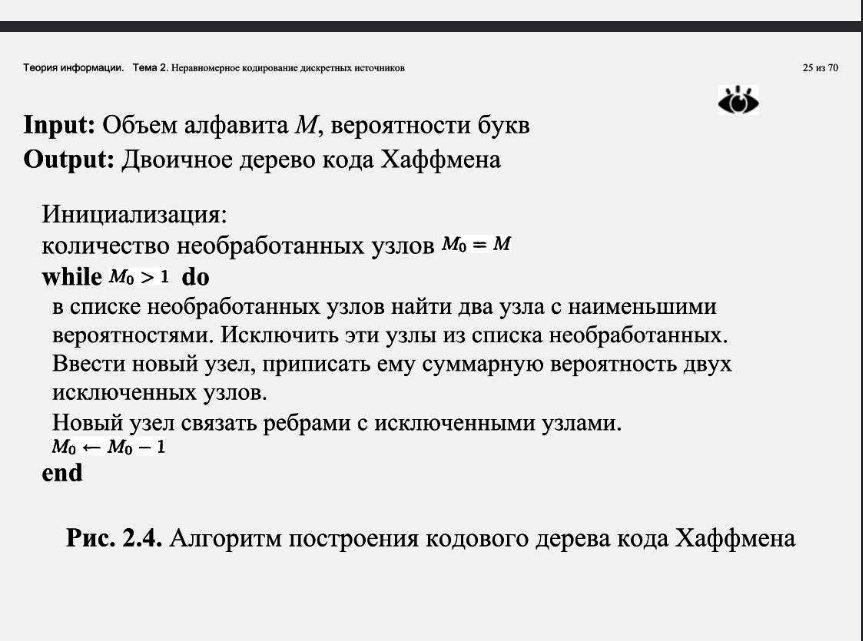
\includegraphics[width=90mm]{huffman_1.png}
\caption{Алгоритм кодирования по Хаффману}
\end{figure}

\begin{figure}[ht!]
\centering
    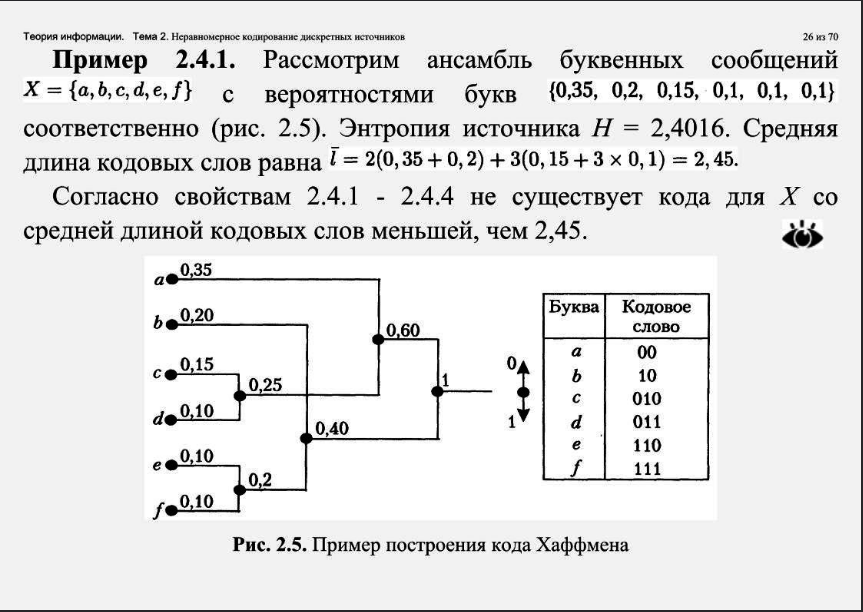
\includegraphics[width=90mm]{huffman_2.png}
\caption{Пример кодирования по Хаффману}
\end{figure}

\bigskip
\textbf{37. Свойства кодовых последовательностей (свойства 2.4.1- 2.4.4 с доказательством).} \\

\textbf{Свойство 2.4.1.} Если \(p_i < p_j\), то \(l_i \geq l_j\)

\textbf{Доказательство.} Свойство доказывается методом «от противного». Предположим, что \(l_i < l_j\). Рассмотрим другой код \(C'\), в котором сообщению \(x_i\) соответствует слово \(c_j\), а сообщению \(x_j\) - слово \(c_i\). Тогда средняя длина кодовых слов для кода \(C'\) меньше, чем для кода \(C\), что противоречит предположению об оптимальности кода \(C\).

\textbf{Свойство 2.4.2.} Не менее двух кодовых слов имеют одинаковую длину \(l_M = max_m l_m\)

\textbf{Доказательство.} Если предположить, что имеется только одно слово максимальной длины, то соответствующее кодовое дерево будет неполным. Слово максимальной длины можно будет сделать короче по меньшей мере на 1 символ. При этом уменьшится средняя длина кодовых слов, что противоречит предположению об оптимальности кода.

\textbf{Свойство 2.4.3.} Среди кодовых слов длиной \(l_M = max_m l_m\) найдутся два слова, различающиеся только в одном последнем символе.

\textbf{Доказательство.} Согласно предыдущему свойству, два слова длиной \(l_M\) существуют в любом оптимальном коде. Рассмотрим концевой узел, соответствующий одному из слов максимальной длины. Чтобы дерево было полным, должен существовать узел, имеющий общий предшествующий узел с данным узлом. Соответствующие двум концевым вершинам кодовые слова имеют одинаковую длину \(l_M\) и различаются в одном последнем символе.

Для рассматриваемого ансамбля \(X = \{1,...,M\}\) и некоторого кода \(C\), удовлетворяющего свойствам 2.4.1 - 2.4.3, введем вспомогательный ансамбль \(X' = \{1,...,M - 1\}\) сообщениям которого сопоставим вероятности \(\{p_1',...,p_{M-1}'\}\) следующим образом: \(p_1' = p_1, ..., p_{M-2}' = p_{M-2}, p_{M-1}' = p_{M-1} + p_M\).

Из кода \(C\) построим код \(C'\) для ансамбля \(X'\), приписав сообщениям \(x_1',\ldots,x_{M-2}'\) те же кодовые слова, что и в коде \(C\), то есть \(c_i' = c_i, i = 1,\ldots,M - 2\), а сообщению \(x_{M-1}'\) - слово \(c_{M-1}'\), представляющее собой общую часть слов \(c_{M-1}\) и \(c_M\) (согласно свойству 2.4.3, эти два кодовых слова различаются только в одном последнем символе).

\textbf{Свойство 2.4.4.} Если код \(C'\) для \(X'\) оптимален, то код \(C'\) оптимален для \(X\).

\textbf{Доказательство.} Длины кодовых слов кодов \(C\) и \(C'\) по построению связаны соотношениями оптимального неравномерного кода. После выполнения алгоритма будет получено кодовое дерево кода, который имеет наименьшую возможную среднюю длину кодовых слов.
\begin{displaymath}
l_m = \left\{ \begin{array}{ll}
    l_m' & \textrm{при \(m \leq M - 2\),}\\
    l_{M-1}' + 1 & \textrm{при \(m \leq M - 1, M\),}\\
  \end{array} \right.
\end{displaymath}

Отсюда:
\begin{displaymath}
    \begin{aligned}
    \bar{l} = \sum_{m=1}^{M} p_m l_m = \sum_{m=1}^{M-2} p_m l_m + p_{M-1} l_{M-1} + p_{M} l_{M} = \sum_{m=1}^{M-2} p_m l_m + (p_{M-1} + p_M)(l_{M-1}' + 1) \\
        = \sum_{m=1}^{M-2} p_m' l_m' + p_{M-1}' l_{M-1}' + p_{M_1} + p_{M} = \sum_{m=1}^{M-1} p_m' l_m' + p_{M_1} + p_{M} = \bar{l} + p_{M_1} + p_{M} \\
    \end{aligned}
\end{displaymath}
где \(\bar{l} = \displaystyle\sum_{m=1}^{M-1} p_m' l_m'\) - средняя длина кодовых слов кода \(C'\).

Последние два слагаемых в правой части не зависят от кода, поэтому код, минимизирующий \(\bar{l}'\), одновременно обеспечивает
минимум для \(\bar{l}\).

Рассмотренные свойства оптимальных префиксных кодов сводят задачу построения кода объемом \(M\) к задаче построения кодов объемом \(M' = M - 1\). Таким образом, получается рекуррентное правило построения кодового дерева.


\bigskip
\textbf{38. Избыточность кода Хаффмена (теорема 2.6).} \\

Разность \(r = \bar{l} - H\) называется избыточностью неравномерного кода.

Она показывает степень «несовершенства» кода в том смысле, что при кодировании с избыточностью \(r\) на каждое сообщение тратится на \(r\) бит больше, чем в принципе можно было бы потратить, если использовать теоретически наилучший (возможно, нереализуемый) способ кодирования.

\textbf{ТЕОРЕМА 2.6.} (Р. Галлагер). Пусть \(p_1\) - наибольшая из вероятностей сообщений конечного дискретного ансамбля. Тогда избыточность кода Хаффмена для этого ансамбля удовлетворяет неравенствам
\begin{displaymath}
r \leq \left\{ \begin{array}{ll}
    p_1 + \sigma & \textrm{при \(p_1 < 1/2\),}\\
    2 - \eta(p_1) - p_1 & \textrm{при \(p_1 \geq 1/2\),}\\
  \end{array} \right.
\end{displaymath}
где \(\eta(x) = -x \log x - (1 - x)\log(1 - x)\) - энтропия двоичного ансамбля, и
\begin{displaymath}
    \sigma = 1 - \log e - \log \log e \approx 0.08607
\end{displaymath}

\bigskip
\textbf{39. Оценка избыточности Галлагера и Манстеттена для кода Хаффмена.} \\

Оценка Галлагера довольно точна в широком диапазоне значений \(p_1\).
Для ансамбля с вероятностями сообщений \(\{1/3, 1/3, 1/3, 0\}\) имеем
оценку 0,419. Истинная избыточность кода Хаффмена для этого
источника 0,417. Для троичного источника с распределением
вероятностей \(\{p_1, 1 - p_1,0\}\) оценка теоремы дает точный результат.

НО существенно улучшить оценку, располагая только значением \(p_1\),
довольно трудно. В то же время для примера 2.4.1 теорема 2.6 дает
оценку \(r \leq 0,35 + 0,0861 = 0,4361\) - при том, что истинное значение
избыточности \(r = 2,45 - 2,4016 = 0,0484\).

Оценка Галлагера недостаточно точна при \(p_1 < 0,5\).

Провел оценку точной границы для всех значений \(p_1\) Манстеттен (рис. 2.6).

\begin{figure}[ht!]
\centering
    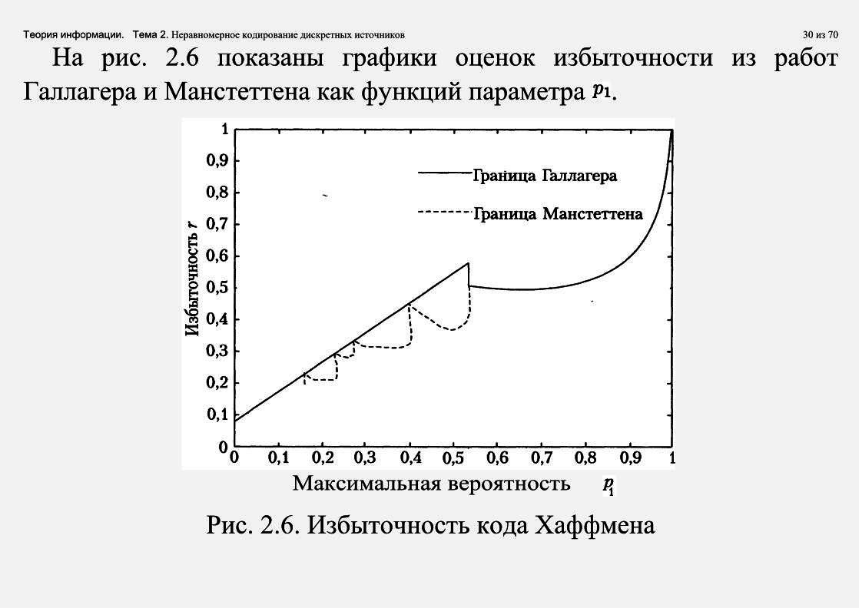
\includegraphics[width=90mm]{gallager_mark.png}
\caption{Оценка избыточности по Галлагеру и Манстеттену}
\end{figure}

\bigskip
\textbf{40. Код Шеннона (арифметический алгоритм построения, пример).} \\

Рассмотрим источник, выбирающий буквы из множества \(X = \{1,...,M\}\) с вероятностями \(\{p_1,...,p_M\}\) Считаем, что буквы упорядочены по убыванию вероятностей, то есть \(p_1 \geq p_2 \geq \ldots \geq p_M\). Сопоставим, кроме того, каждой букве так называемую кумулятивную вероятность по правилу
\begin{displaymath}
    q_1 = 0, q_2 = p_1, \ldots, q_M = \sum_{i=1}^{M-1} p_i
\end{displaymath}

Кодовым словом кода Шеннона для сообщения с номером \(m\) является двоичная последовательность, представляющая собой первые \(l_m = \lceil -\log p_m \rceil\) разрядов после запятой в двоичной записи числа \(q_m\).

Смотреть рисунки 5 и 6.

\begin{figure}[hp]
\centering
    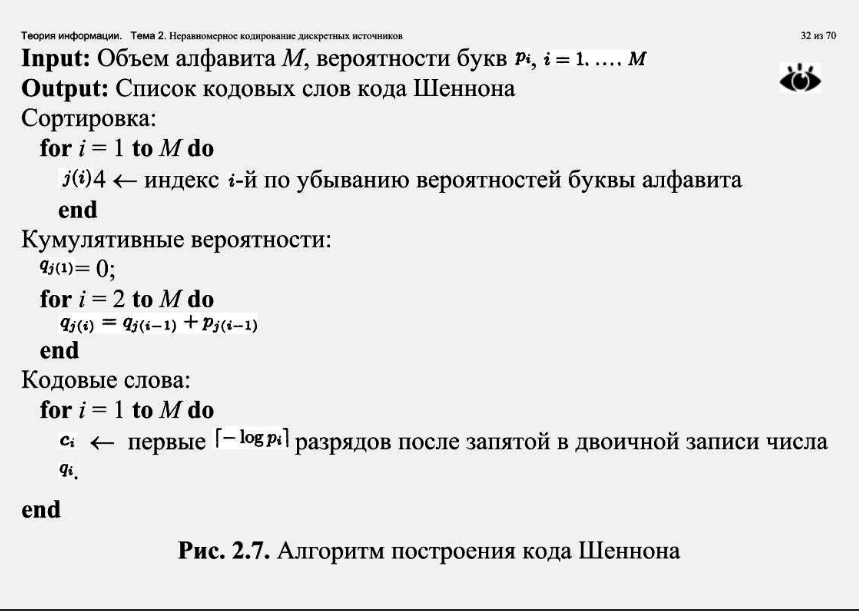
\includegraphics[width=90mm]{shennon_alg.png}
\caption{Алгоритм кодирования по Шеннону}
\end{figure}

\begin{figure}[hp]
\centering
    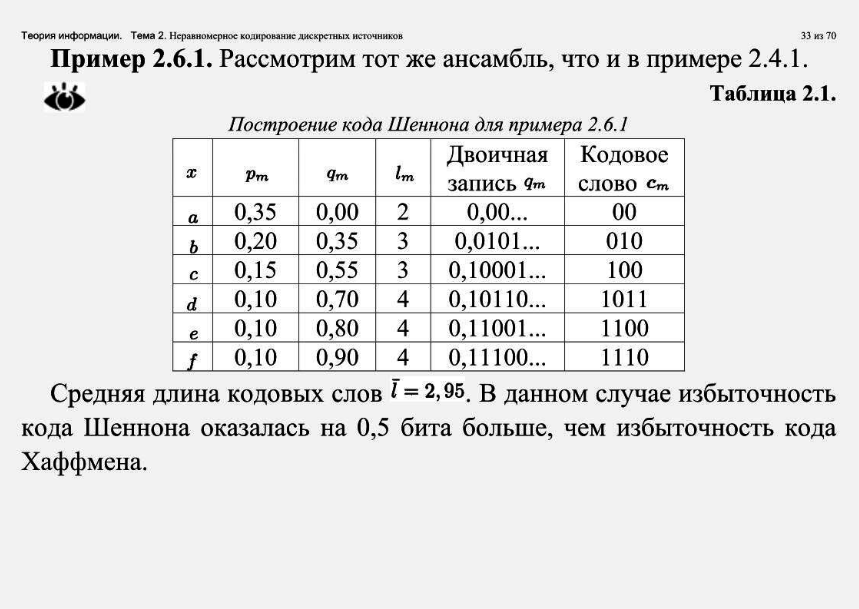
\includegraphics[width=90mm]{shennon_example.png}
\caption{Пример кодирования по Шеннону}
\end{figure}


\bigskip
\textbf{41. Графическая интерпретация кода Шеннона.} \\

\begin{figure}[hp]
\centering
    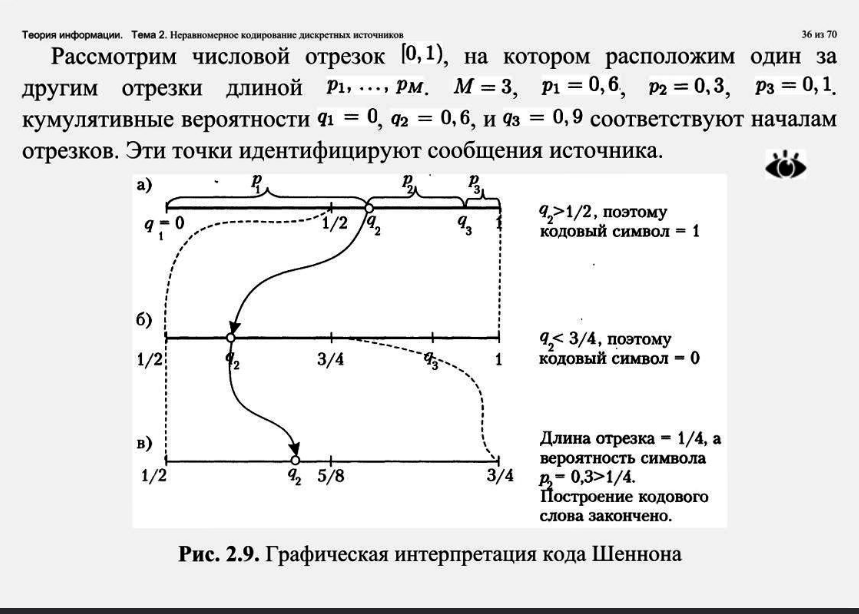
\includegraphics[width=90mm]{shennon_inter.png}
\caption{Графическая интерпретация кода Шеннона}
\end{figure}

Смотреть рисунок 7.

Если требуется закодировать сообщение с номером \(m = 2 (q_2 = 0.6)\):

1. На первом шаге передачей кодового символа 0 либо 1 кодер указывает, в какой половине отрезка \([0,1)\) (левой или правой) находится начало соответствующего отрезка. Передается 1, поскольку значение правее середины исходного отрезка (\(q = 0.5\)). В результате область возможных положений передаваемой точки уменьшается вдвое.

2. На следующем шаге передается символ 0, так как точка находится в левой половине интервала (относительно \(q = 0.75\)) и длина интервала неопределенности уменьшается до 1/4.

3. После второго шага в интервале неопределенности осталась только одна точка, поэтому передача может быть завершена (длина интервала равна 1/4, что меньше длины кратчайшего прилегающего отрезка 0.3) - именно поэтому гарантируется единственность точки, а значит, и однозначность декодирования.


\bigskip
\textbf{42. Код Гилберта-Мура (алгоритм построения кода, пример).} \\

При построении кода Шеннона требуется упорядоченность сообщений по убыванию вероятностей. В алгоритме построения кода Шеннона наиболее трудоемкой частью является сортировка букв входного алфавита. Сильно упростить построение кода, можно, если модифицировать кодирование таким образом, чтобы упорядоченность не требовалась.

Предположим, что вероятности не упорядочены и при кодировании сообщения с номером \(m\) нужно учитывать не только вероятность (длину отрезка) \(p_m\), но и длину предшествующего отрезка \(p_{m-1}\), которая может быть очень маленькой, почти нулевой (тогда длина слова будет большой, даже если вероятность \(p_m\)велика).

Для того, чтобы избавиться от влияния \(p_{m-1}\) нужно соответствующую сообщению точку переместить из начала отрезка (точка \(q_m\)) в его середину (точка \(q_m + p_m / 2\)), а длину кодового слова \(l_m\) выбрать так, чтобы к концу передачи кодового слова интервал неопределенности был не больше \(p_m / 2\). Эти \(l_m\) бит и будут кодовым словом кода Гилберта-Мура!

Определим код Гилберта-Мура формально.

Рассмотрим источник, выбирающий буквы из алфавита \(X = \{1,...,M\}\) с вероятностями \(\{p_1,...,p_M\}\). Сопоставим каждой букве \(m = 1,\ldots,M\) кумулятивную вероятность \(q_m = \sum_{i=1}^{m-1} p_i\) и вычислим для каждой буквы величину \(\sigma_m\) по формуле
\begin{displaymath}
    \sigma_m = q_m + \frac{p_m}{2}
\end{displaymath}

Кодовым словом кода Гилберта-Мура для \(x_m\) является двоичная
последовательность, представляющая собой первые \(l_m = \lceil -\log(p_m/2) \rceil\)
разрядов после запятой в двоичной записи числа \(\sigma_m\).

\begin{figure}[hb]
\centering
    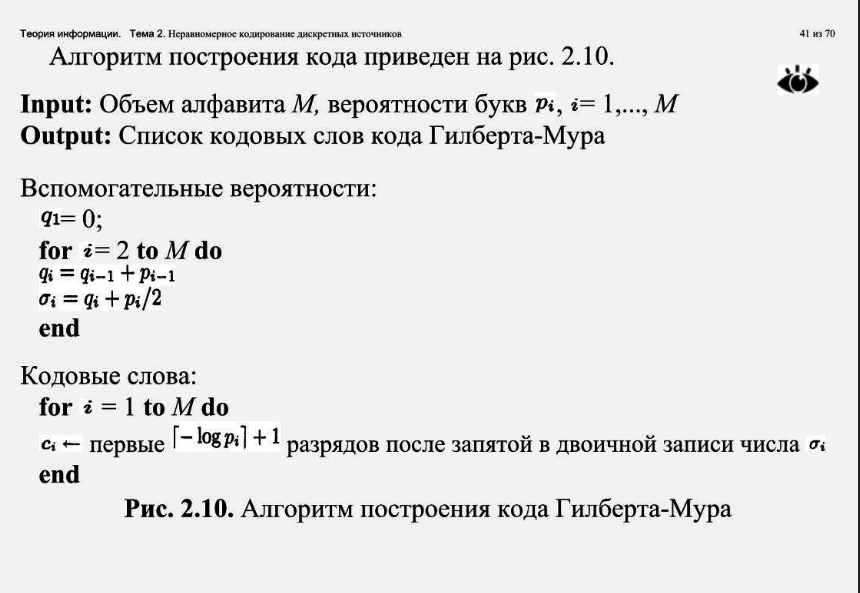
\includegraphics[width=90mm]{gilbert_alg.png}
\caption{Алгоритм построения кода Гилберта-Мура}
\end{figure}

\begin{figure}[pt]
\centering
    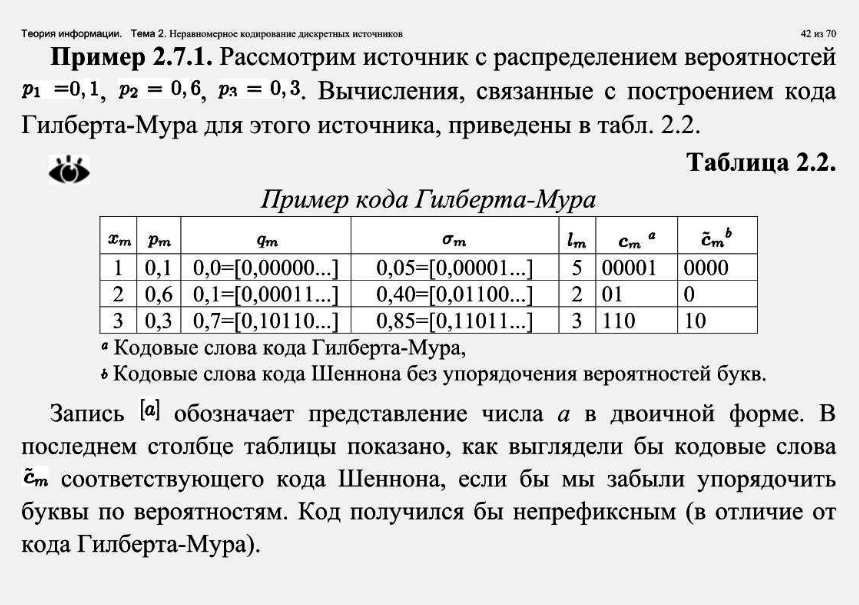
\includegraphics[width=90mm]{gilbert_example.png}
\caption{Пример построения кода Гилберта-Мура}
\end{figure}


\vskip5cm
\textbf{43. Однозначность декодируемости кода Гилберта-Мура.} \\

Докажем однозначную декодируемость кода Гилберта-Мура в общем случае. Выберем сообщения с номерами \(i\) и \(j\), \(i < j (\sigma_j > \sigma_i)\). Нужно доказать, что соответствующие слова \(c_i\) и \(c_j\); различаются хотя бы в одном из первых \(min\{l_i, l_j\}\) кодовых символов.
\begin{displaymath}
    \begin{aligned}
    \sigma_j - \sigma_i = \sum_{h=1}^{j-1} p_h + \frac{p_j}{2} - \sum_{h=1}^{i-1} p_h - \frac{p_i}{2} = \\
    = \sum_{h=1}^{j-1} p_h + \frac{p_j - p_i}{2} \geq p_i + \frac{p_j - p_i}{2} = \\
    = \frac{p_j + p_i}{2} = \frac{max\{p_i, p_j\}}{2}
    \end{aligned}
\end{displaymath}

Длина слова и его вероятность связаны соотношением
\begin{displaymath}
    l_m = \lceil -\log(p_m / 2) \rceil \geq -\log \frac{p_m}{2}
\end{displaymath}
\begin{displaymath}
    \sigma_j - \sigma_i \geq \frac{max\{p_i, p_j\}}{2} \geq 2^{-min\{l_i, l_j\}}
\end{displaymath}
слова \(c_i\) и \(c_j\) различаются в одном из первых \(min\{l_i, l_j\}\) двоичных символов, поэтому ни одно из двух слов не может быть началом другого.

Поскольку все слова кода Гилберта-Мура ровно на 1 длиннее слов кода Шеннона, получаем оценку средней длины кодовых слов \(\bar{l} < H + 2\).


\bigskip
\textbf{44. Неравномерное кодирование для стационарного источника.} \\

Рассмотрим последовательность \(x_1, x_2, \ldots, x_i \in X = \{x\}\), наблюдаемую на выходе дискретного стационарного источника, для которого известно вероятностное описание - можно вычислить все многомерные распределения вероятностей и по ним - энтропию на сообщение \(H = H_{\infty}(X)\).

Пусть указан некоторый способ кодирования, строящий (для любых \(n\) для каждой последовательности \(x \in X^n\)) на выходе источника кодовое слово \(c(x)\) длиной \(l(x)\)). Тогда средняя скорость кодирования для блоков длиной \(n\) определяется как
\begin{displaymath}
    \bar{R_n} = \frac{1}{n}\textbf{M}[l(x)]
\end{displaymath}
бит/сообщение источника.

Подбирая длину блоков, при которой средняя скорость будет наименьшей, получаем следующее определение для средней скорости кодирования:
\begin{displaymath}
    \bar{R} = \inf_{n}\bar{R_n}
\end{displaymath}

Здесь используется нижняя грань (inf) вместо минимума, поскольку наименьшее значение скорости может достигаться в пределе при \(n \to \infty\).

Рассматриваемое кодирование - FV-кодирование (fixed-to-variable), поскольку блоки из фиксированного числа сообщений \(n\) кодируются кодовыми словами переменной длины.


\bigskip
\textbf{45. Средняя скорость кодирования для дискретного стационарного источника (теорема 2.7 с доказательством).} \\

\textbf{ТЕОРЕМА 2.7.} Для дискретного стационарного источника с энтропией на сообщение \(H\) для любого FV-кодирования имеет место неравенство
\begin{displaymath}
    \bar{R} \geq H
\end{displaymath}

\textbf{Доказательство.} Рассмотрим множество \(X^n\). К его элементам применим теорему побуквенного кодирования
\begin{displaymath}
    \textbf{M}[l(x)] \geq H(X^n) = nH_n(X) \geq nH_{\infty}(X) = nH
\end{displaymath}

Второе неравенство здесь выполняется так как \(H_n(X)\) не возрастает с увеличением \(n\). Тогда
\begin{displaymath}
    \bar{R_n} \geq H
\end{displaymath}
при любых \(n\).
\begin{displaymath}
    \bar{R} = \inf_{n}\bar{R_n} \geq H
\end{displaymath}


\bigskip
\textbf{46. Прямая теорема кодирования для дискретного стационарного источника (теорема 2.8 с доказательством).} \\

\textbf{ТЕОРЕМА 2.8.} Для дискретного стационарного источника с энтропией на сообщение \(H\) и для любого \(\delta > 0\) существует способ неравномерного FV-кодирования такой, для которого
\begin{displaymath}
    \bar{R} \leq H + \delta
\end{displaymath}

\textbf{Доказательство.} Воспользовавшись прямой теоремой побуквенного кодирования для ансамбля \(X^n\), мы можем утверждать, что для некоторого побуквенного кода имеет место неравенство
\begin{displaymath}
    \textbf{M}[l(x)] \leq H(X^n) + 1 = nH_n(X) + 1
\end{displaymath}

По определению предела числовой последовательности существует достаточно большое число \(n_1\) такое, что при всех \(n \geq n_1\) имеет место неравенство
\begin{displaymath}
    |H_n(X) - H| \leq \frac{\delta}{2}, (2.8)
\end{displaymath}

из которого следует, что
\begin{displaymath}
    H_n(X) \leq H + \frac{\delta}{2}, n > n_1, (2.9)
\end{displaymath}

Найдем \(n_2\) такое, что при \(n \geq n_2\) имеет место неравенство
\begin{displaymath}
    \frac{1}{n} \leq \frac{\delta}{2}, (2.10)
\end{displaymath}

С учетом (2.9) и (2.10) из (2.8) получаем при \(n \geq max\{n_1, n_2\}\)
\begin{displaymath}
    \bar{R} = \inf_{m}\bar{R_m} \geq \bar{R_n} = \frac{\textbf{M}[l(x)]}{n} \leq H_n(X) + \frac{1}{n} \leq H + \frac{\delta}{2} + \frac{\delta}{2} = H + \delta
\end{displaymath}

Выбрав достаточно большую длину блоков \(n\) и применив к блокам побуквенное кодирование, мы получим кодирование со средней скоростью
\begin{displaymath}
    H \leq \bar{R} \leq H + o(n)
\end{displaymath}
где \(o(n) \to 0\) при \(n \to \infty\).

Но наблюдается экспоненциальный рост сложности при росте длины блоков \(n\).

\bigskip
\textbf{47. Арифметическое кодирование (алгоритм построения кода, пример).} \\

Сам алгоритм является почти тривиальным обобщением кода Шеннона на последовательности. Рассмотрим дискретный постоянный источник, выбирающий сообщения из множества \(X = \{1,...,M\}\) с вероятностями \(\{p_1,...,p_M\}\).

Обозначим через \(\{q_1,...,q_M\}\) кумулятивные вероятности сообщений. Необходимо закодировать последовательности множества \(X^n = \{x\}\). Для записи подпоследовательности \((x_i,...,x_j)\) в последовательности \(x = (x_1,...,x_n)\) будем использовать обозначение \(x_i^j\).

Необхоимо применить к ансамблю - \(X^n = \{x\}\) достаточно простой и эффективный побуквенный код. Упрощение состоит в том, что ни кодер, ни декодер не хранят и не строят всего множества из \(|X^n|\) кодовых слов. Вместо этого при передаче конкретной последовательности \(x\) кодером вычисляется кодовое слово \(c(x)\) только для данной последовательности \(x\). Правило кодирования, конечно, известно декодеру, и он восстанавливает \(x\) по \(c(x)\), не имея полного списка кодовых слов.

Можно использовать код Шеннона или код Гилберта-Мура. Однако использование кода Шеннона предполагает упорядоченность сообщений по убыванию вероятностей. При больших \(n\) сложность упорядочения окажется очень большой, поэтому можно использовать только код Гилберта-Мура.

В соответствии с правилом построения кода Гилберта-Мура кодовое слово формируется по вероятности \(p(x)\) и кумулятивной вероятности \(q(x)\) как первые \(l(x) = \lceil -\log(p(x)) + 1\rceil\) разрядов после точки в двоичной записи числа \(\sigma(x) = q(x) + p(x)/2\).

Чтобы вычислить \(q(x)\), необходимо определить нумерацию последовательностей из \(X^n\). Будем использовать лексикографический (алфавитный) порядок для последовательностей. Запись \(y \prec x\) будет означать, что \(y\) лексикографически предшествует \(x\).

Понятие лексикографического порядка определяется следующим образом.

Для последовательностей длиной 1 (для отдельных сообщений из \(X\)) мы считаем, что сообщение с меньшим номером предшествует сообщению с большим номером. Если, например, элементы \(X\) - числа, то \(x \prec x'\), если \(x < x', x,x' \in X\).

Для двух последовательностей \(x = (x_1,...,x_n)\), \(y = (y_1,...,y_n)\) обозначим через \(i\) наименьший индекс такой, что \(x_i \neq y_i\). Тогда \(y \prec x\), если \(y_i \prec x_i\).

Лексикографический порядок - это порядок, который обычно используется при составлении словарей.

Основная задача состоит в вычислении кумулятивной вероятности
\begin{displaymath}
    q(x) = \sum_{y \prec x} p(y)
\end{displaymath}

Для источника без памяти вероятности последовательностей \(p(x)\):
\begin{displaymath}
    p(x) = \prod_{i=1}^{n} p(x_i)
\end{displaymath}

Выведем рекуррентную формулу для \(q(x)\). Для этого выразим вероятность \(q(x_1^n)\) через \(q(x_1^{n-1})\);
\begin{displaymath}
    q(x_1^n) = q(x_1^{n-1}) + p(x_1^{n-1})q(x_n)
\end{displaymath}
\begin{displaymath}
    p(x_1^n) = p(x_1^{n-1})p(x_n)
\end{displaymath}

Здесь каждая пара значений \((q(x_1^i), p(x_1^i))\) используется ровно на одном шаге при вычислении следующей пары \((q(x_1^{i+1}), p(x_1^{i+1}))\).

При реализации арифметического кодирования вновь вычисленные значения записываются в те же ячейки памяти, в которых находились предыдущие значения.

\begin{figure}[ht!]
\centering
    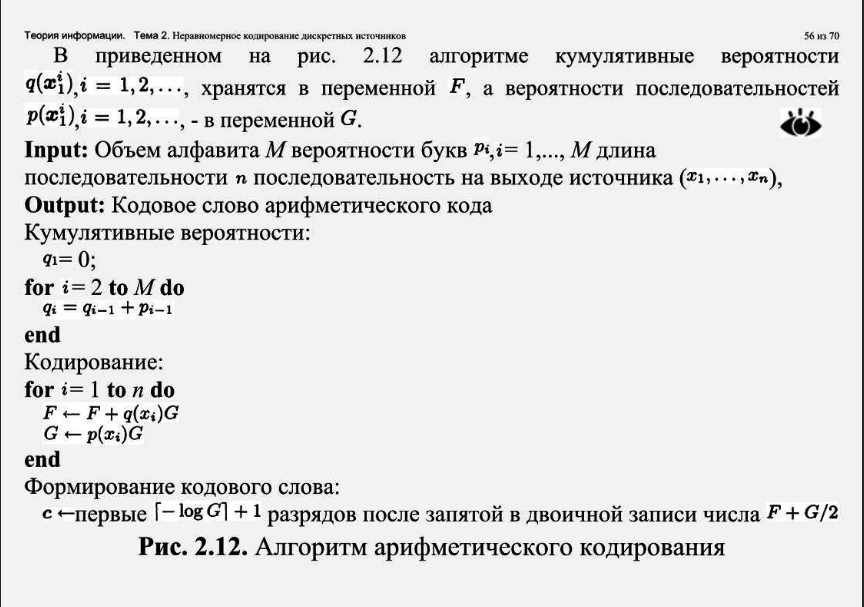
\includegraphics[width=90mm]{aryph_alg.png}
\caption{Алгоритм построения арифметического кода}
\end{figure}

\begin{figure}[pt]
\centering
    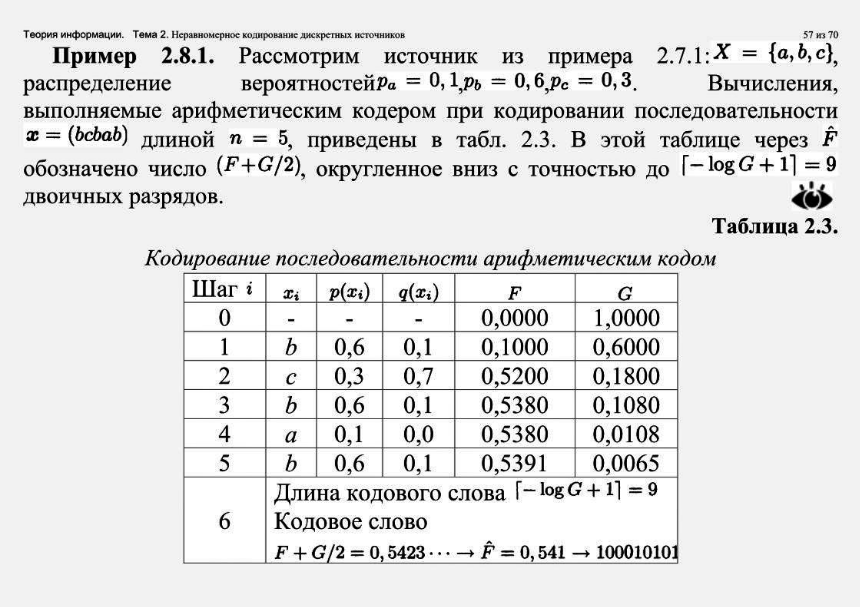
\includegraphics[width=90mm]{aryph_example.png}
\caption{Пример построения арифметического кода}
\end{figure}

\bigskip
\textbf{48. Сложность реализации кодирования арифметического кода} \\

Сложность кодирования. Из описания алгоритма следует, что на каждом шаге кодирования выполняется одно сложение и два умножения. Кажется, что сложность кодирования последовательности из \(n\) сообщений пропорциональна \(n\). Однако, это неверно, поскольку на каждом шаге линейно растет сложность выполнения самих операций сложения и умножения, так как нарастает число двоичных разрядов, необходимых для записи операндов.

Для представления вероятностей \(\{p_1,...,p_M\}\) используются числа разрядности \(d\). После первого шага кодирования точное представление F и G потребует \(2d\) разрядов. После \(n\) шагов кодирования кодер и декодер будут работать (в худшем случае) с числами разрядности \(nd\), и, следовательно, суммарная сложность имеет порядок
\begin{displaymath}
    d + 2d + \ldots + nd = \frac{n(n + 1)}{2}d
\end{displaymath}

Сложность арифметического кодирования пропорциональна \(n^2\)

На самом деле все же возможна практическая реализация арифметического кодирования со сложностью \(n\) (за счет потери в точности вычислений).

Если в качестве модели источника рассматривается простая цепь
Маркова, то алгоритм кодирования остается прежним - за тем
исключением, что вместо одномерных вероятностей \(p(x_i)\) и \(q(x_i)\) нужно
использовать условные вероятности  \(p(x_i|x_{i-1})\) и
\begin{displaymath}
    q(x_i|x_{i-1}) = \sum_{y \prec x_i} p(y|x_{i-1})
\end{displaymath}

\bigskip
\textbf{49. Декодирование арифметического кода (алгоритм декодирования, пример).} \\

При арифметическом кодировании и использовании последовательностей большой длины \(n\) возникают следующие проблемы:
\begin{itemize}
    \item арифметическое кодирование требует большой (в пределе - бесконечной) точности вычислений, что ведет к недопустимо высокой сложности реализации;
    \item для формирования кодового слова формально необходима вся последовательность сообщений, что приводит к недопустимо большой задержке кодирования, равной длине кодируемой последовательности.
\end{itemize}

Обе эти проблемы преодолимы. Решение состоит в том, что та часть данных, которая не участвует в дальнейших вычислениях и уже не влияет на окончательный результат, может быть исключена из вычислений и сразу выдана на выход кодера. При этом уменьшается сложность вычислений и задержка кодирования.

\begin{figure}[ht!]
\centering
    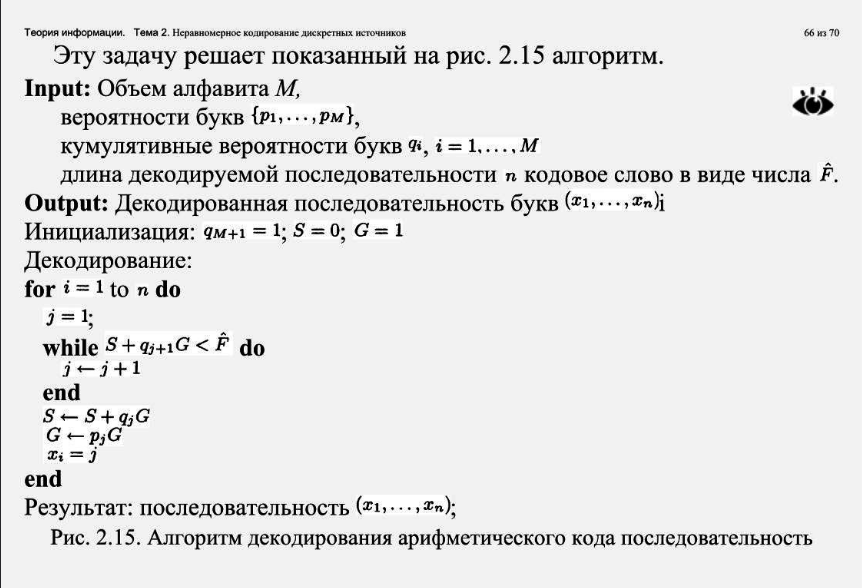
\includegraphics[width=90mm]{aryph_decode_alg.png}
\caption{Алгоритм декодирования арифметического кода}
\end{figure}

\begin{figure}[h!]
\centering
    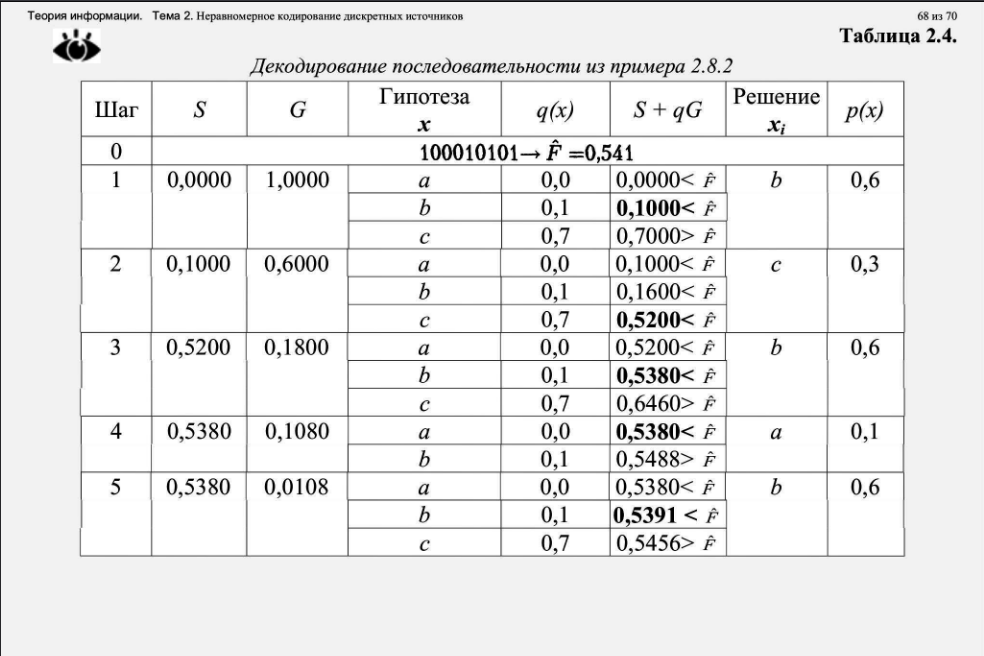
\includegraphics[width=90mm]{aryph_decode_example.png}
\caption{Пример декодирования арифметического кода}
\end{figure}

\vskip3cm
\textbf{50. Формула, определяющая число сочетаний.} \\

Число различных подмножеств:
\begin{displaymath}
        C_M^n = \binom{M}{n} = \frac{A_M^n}{P_n} = \frac{M(M - 1) \times ... \times (M - n + 1)}{n!} = \frac{M!}{n!(M - n)!}
\end{displaymath}
Это количество называют числом сочетаний из \(M\) элементов по \(n\).

\bigskip
\textbf{51. Композиция последовательности.} \\

Композицией последовательности \(x\) называется вектор \(\tau(x) = (\tau_0(x) ,..., \tau_{M-1}(x))\) в котором \(\tau_i(x)\) обозначает число элементов \(x_i = i\) в последовательности \(x = (x_1,...,x_n)\).

Необходимо определить число последовательностей \(x\) с заданной композицией \(\tau = (\tau_0 ,..., \tau_{M-1})\).

Положим \(M = 3\) и найдем число последовательностей длины \(n\) с композицией \(\tau = (\tau_0, \tau_1, \tau_2)\), \(n = \tau_0 + \tau_1 + \tau_2\).

Зафиксируем некоторое расположение нулей (это можно сделать \(\binom{n}{\tau_0}\) способами) и подсчитаем количество различных расположений \(\tau_1\) единиц на оставшихся \(n - \tau_0\) позициях. Это число равно \(\binom{n - \tau_0}{\tau_1}\).

Поскольку каждому расположению нулей соответствует именно такое количество расположений единиц, общее число последовательностей
\begin{displaymath}
    N(\tau) = \binom{n}{\tau_0}\binom{n - \tau_0}{\tau_1} = \frac{n!}{\tau_0!(n - \tau_0)!} \frac{(n - \tau_0)!}{\tau_1!(n - \tau_0 - \tau_1)!} = \frac{n!}{\tau_0!\tau_1!\tau_2!}
\end{displaymath}

Аналогично для алфавита произвольного объема \(M\)справедлива формула
\begin{displaymath}
    N(\tau) =  \frac{n!}{\tau_0!...\tau_{M-1}!}
\end{displaymath}

\bigskip
\textbf{52. Представления натурального числа (лемма 3.1 с доказательством).} \\

\textbf{ЛЕММА 3.1.} Натуральное число \(n\) может быть представлено в
виде суммы \(M\) неотрицательных целых слагаемых \(\binom{n+M-1}{M-1}\) способами.

\textbf{Доказательство.} Будем записывать последовательность из \(j\) нулей в виде \(0^j\) Каждому разбиению числа \(n\) на целые слагаемые \(a_1 + ... + a_M = n...\) соответствует двоичная последовательность вида \((0^{a_1}1, 0^{a_2}1,...,0^{a_M})\). Длина последовательности равна \(n + M - 1\), а вес равен \(M - 1\).

Тогда число разбиений равно числу таких последовательностей, которое, в свою очередь, равно числу двоичных последовательностей длиной \(n + M - 1\), содержащих \(M - 1\) единиц, которое равно \(\binom{n+M-1}{M-1}\).

\bigskip
\textbf{53. Рекуррентная формула вычисления числа двоичных последовательностей длиной n весом w.} \\

Число \(\binom{n}{\omega}\) можно интерпретировать как число двоичных последовательностей длиной \(n\) весом \(\omega\). Справедлива рекуррентная формула
\begin{displaymath}
    \binom{n + 1}{\omega} = \binom{n}{\omega} + \binom{n}{\omega - 1}
\end{displaymath}

Тогда любая последовательность длиной \(n + 1\) весом \(\omega\) может быть получена либо из последовательности длиной \(n\) весом \(\omega\) дописыванием нуля, либо из последовательности длиной \(n\) весом \(\omega - 1\) дописыванием единицы.

Применим эту формулу ко второму слагаемому. Выполнив это рекурсивно получим
\begin{displaymath}
    \binom{n + 1}{\omega} = \binom{n}{\omega} + \binom{n - 1}{\omega - 1} + ... + \binom{n - \omega + 1}{1}
\end{displaymath}

\bigskip
\textbf{54. Двухпроходное побуквенное кодирование.} \\

Будем считать, что источник выбирает сообщения из множества \(X = \{0,...,M-1\}\) Пусть \(x = (x_1,...,x_n)\) — последовательность на выходе источника. Множество сообщении \(X\) и длину последовательности считаем заранее известными кодеру и декодеру.

На практике длина последовательности либо передается отдельно в заголовке файла некоторым стандартным способом, либо в алфавите источника имеется специальный символ, указывающий на завершение файла. В любом случае для всех методов универсального кодирования проблема конца файла решается одинаковым способом, и от способа ее решения сравнительные характеристики алгоритмов не зависят.

Рассмотрим универсальное кодирование для класса источников без памяти с неизвестным распределением вероятностей на буквах источника.

Тогда для решения задачи кодер просматривает последовательность и определяет число появлений \(\tau_n(a)\) каждой буквы \(a \in X\) в последовательности \(x\) длины \(n\).

Затем, используя полученную информацию, кодер вычисляет оценки вероятностей сообщений и строит по ним некоторый код для множества \(X\).

На втором проходе этот код используется для кодирования последовательности сообщений источника. Кодовое слово состоит из двух частей \(c(x) = (c_1(x), c_2(x))\). Первая часть \(c_1(x)\) содержит информацию об использованном коде, вторая \(c_2(x)\) - собственно закодированную последовательность букв.

Декодер сначала по \(c_1(x)\) строит код, затем по \(c_2(x)\) восстанавливает одно за другим закодированные сообщения.

\bigskip
\textbf{55. Подсчет информационного объема для описания двоичного дерева (лемма 3.2).} \\

\textbf{ЛЕММА 3.2.} Полное кодовое дерево, имеющее \(M\) концевых вершин, имеет \(M - 1\) промежуточных вершин. Для полного описания дерева достаточно \(2M - 1\) бит.

\bigskip
\textbf{56. Средняя скорость кодирования при двухпроходном кодировании (теорема 3.3 с доказательством).} \\

\textbf{ТЕОРЕМА 3.3.} При двухпроходном кодировании с использованием кода Хаффмена дискретного постоянного источника с объемом алфавита \(M\) и энтропией \(H\) средняя скорость кодирования удовлетворяет неравенству
\begin{displaymath}
    \bar{R} \leq H + 1 + \frac{1}{n}(M\log M + 3M - 1)
\end{displaymath}

\textbf{Доказательство.} Для заданной последовательности \(x\) через \(l_1(x)\) и \(l_2(x)\) обозначаем длину первой и второй частей кодового слова соответсвенно.

Информация о коде может быть разбита на две части:

1) информация о кодовом дереве и информация о том, какая из букв соответствует каждой вершине кодового дерева. Длина описания кодового дерева может быть оценена с использованием леммы 3.2. \\
Указание буквы для одной вершины потребует не более \\
\begin{displaymath}
    \lceil \log M \rceil \leq \log M + 1 
\end{displaymath}
бит.

В результате имеем оценку:
\begin{displaymath}
    l_1(x) \leq 2M - 1 + M\lceil \log M \rceil \leq M\log M + 3M - 1, (3.20)
\end{displaymath}

2) Длина второй половины кодового слова подсчитывается как:
\begin{displaymath}
    l_2(x) = \sum_{i=1}^{n} l(x_i) = \sum_{x \in X} \tau_n(x) l(x) = n\sum_{x \in X} \frac{\tau_n(x)}{n} l(x) = n\sum_{x \in X} \hat{p}_n(x) l(x) = n\textbf{M}_{\hat{p}_n}[l(x)] \leq n(H(\hat{p}_n) + 1), (3.21)
\end{displaymath}

С учетом (3.20) и (3.21) средняя скорость кодирования для заданной последовательности \(x\) удовлетворяет неравенству
\begin{displaymath}
    \bar{R}(x) = \frac{l(x)}{n} = \frac{l_1(x) + l_2(x)}{n} \leq H(\hat{p}_n) + 1 + \frac{1}{n}(M\log M + 3M - 1)
\end{displaymath}

Следующий шаг доказательства — усреднение по всем последовательностям \(x\). В правой части от \(x\) зависит только энтропия:
\begin{displaymath}
    \textbf{M}[H(\hat{p}_n)] \leq H(\textbf{M}[\hat{p}_n]) = H(p) = H
\end{displaymath}

Здесь неравенство следует из выпуклости \(\cap\) энтропии как функции распределения вероятностей. Для обоснования перехода определим, что
\begin{displaymath}
    \textbf{M}[\hat{p}_n] = p
\end{displaymath}
где через \(p\) обозначен вектор, компонентами которого являются вероятности букв источника.

Иными словами, нужно доказать. что в последнем тождестве равенство имеет место для каждой компоненты
\begin{displaymath}
    \textbf{M}\left[\frac{\tau_n(a)}{n}\right] = p(a), a \in X
\end{displaymath}

Введем индикаторную функцию
\begin{displaymath}
    \chi_a(x) \leq \left\{ \begin{array}{ll}
    1 & \textrm{при \(x = a\),}\\
    0 & \textrm{при \(x \neq a\),}\\
  \end{array} \right.
\end{displaymath}

Кроме того,
\begin{displaymath}
    \textbf{M}[\chi_a(x)] = 1 \times p(a) + 0 \times (1 - p(a)) = p(a) 
\end{displaymath}

Теперь можно записать:
\begin{displaymath}
    \textbf{M}\left[\frac{\tau_n(a)}{n}\right] = \frac{1}{n}\textbf{M}\left[\sum_{i=1}^{n} \chi_a(x_i)\right] = \frac{1}{n}\sum_{i=1}^{n} \textbf{M}[\chi_a(x_i)] = p(a), a \in X
\end{displaymath}

Отсюда следует (3.25) и из него (3.24). В свою очередь. используя (3.24), в результате усреднения в левой и правой частях (3.22) приходим к доказываемому результату (3.19).

\bigskip
\textbf{57. Оценка избыточности нумерационного кодирования. Средняя скорость нумерационного кодирования (теорема 3.4).} \\

\textbf{ТЕОРЕМА 3.4.} При нумерационном кодировании дискретного постоянного источника с объемом алфавита \(M\) и энтропией \(H\) средняя скорость кодирования удовлетворяет неравенству
\begin{displaymath}
    \bar{R} \leq H + \frac{M - 1}{2}\frac{\log(n + 1) + K}{n},
\end{displaymath}
где величина \(K\) не зависит от длины последовательности \(n\).


\bigskip
\textbf{58. Адаптивное кодирование.} \\

Универсальное кодирование без задержки. Кодеру при поступлении на его вход очередного сообщения теперь недоступна информация о сообщениях, которые появятся в будущем. Поэтому способ кодирования текущего сообщения будет зависеть только от того, какими были предыдущие сообщения.

Естественным решением задачи является следующий подход: кодер (и декодер) по последовательности уже переданных сообщений оценивают вероятности возможных значений следующего сообщения и строят для него код в соответствии с этими оценками вероятностей.

Если источник стационарен, то с увеличением длины уже закодированной последовательности оценки вероятностей будут все более точными. У декодера не возникнет проблем с восстановлением данных, поскольку он располагает всей информацией, использованной кодером для построения кода.

В рамках этой схемы есть несколько степеней свободы выбора конкретной модификации алгоритма. В частности, можно менять следующие характеристики:

\begin{itemize}
    \item длину последовательности сообщений, по которой вычисляются оценки вероятностей;
    \item формулы для вычисления оценок вероятностей;
    \item способ кодирования при известных оценках вероятностей.
\end{itemize}

Рассмотрим эти возможности.

Рассмотрим выбор длины «окна», то есть длины последовательности, по которой оцениваются вероятности сообщений.

Увеличение длины окна вообще приводит к росту точности оценок, то есть к повышению эффективности кодирования.

Это верно, если верна гипотеза о стационарности источника. В противном случае выбор короткого окна может оказаться более удачным, поскольку позволит кодеру и декодеру быстрее адаптироваться к изменениям статистических свойств источника.

Более детальный анализ показывает, что и для стационарного источника достаточно выбирать окно, длина которого в несколько раз превышает объем алфавита источника. Дальнейшее увеличение длины окна не приведет заметному уменьшению избыточности. Исходя из этого целесообразным всегда выбирать окна конечной длины.

Однако при этом возрастает сложность кодирования. Так как при «бесконечном окне» (когда окном служит вся предшествующая последовательность сообщений) вся необходимая информация о предшествующих сообщениях хранится в виде счетчиков числа появления различных букв (число счетчиков равно объему алфавита источника).

При окне конечной длины при поступлении от источника новой буквы нужно не только нарастить на 1 значение соответствующего счетчика, но и уменьшить на 1 значение счетчика для той буквы, которая в данный момент времени оказалась за пределами окна.

Для этого придется помнить всю последовательность букв, хранящихся в окне.

С учетом этого вероятности обычно оцениваются по всей предшествующей последовательности.

Выбор формул для оценивания вероятностей и выбор способа кодирования взаимосвязаны.

На первый взгляд оценка вероятности того. что \(x_{n+1} = a\), должна вычисляться по последовательности \(x_1,...,x_n\) по формуле
\begin{displaymath}
    \hat{p}_n(a) = \frac{\tau_n(a)}{n}
\end{displaymath}
где через \(\tau_n(a)\) обозначено число появлений буквы \(a\) в последовательности длины \(n\).

Однако при использовании этой формулы для некоторых букв оценка вероятности окажется равной нулю. Это не вызовет серьезных проблем, если для кодирования используется, например, код Хаффмена. Однако при использовании кодов Шеннона, Гилберта-Мура или арифметического кодирования нулевые значения вероятностей недопустимы.

Оценку вероятностей букв можно провести по формуле
\begin{displaymath}
    \hat{p}_n(a) = \frac{\tau_n(a) + 1}{n + M}
\end{displaymath}

В данной формуле в числителе добавлена единица к счетчику числа появлений букв — тем самым исключаются нулевые вероятности.

К знаменателю нужно добавить объем алфавита, иначе нарушается условие нормировки вероятностей.


\bigskip
\textbf{59. Средняя скорость кодирования при адаптивном арифметическом кодировании (теорема 3.5).}

В лекциях и в вопросах РАЗНЫЕ номера теорем и тем! \\

\textbf{ТЕОРЕМА 3.8.} При адаптивном арифметическом кодировании дискретного постоянного источника с объемом алфавита \(M\) и энтропией \(H\) средняя скорость кодирования удовлетворяет неравенству
\begin{displaymath}
    \bar{R} \leq H + \frac{M}{2}\frac{\log(n + 1) + K}{n}
\end{displaymath}
где величина \(K\) не зависит от длины последовательности \(n\).

\bigskip
\textbf{60. Кодирование A-алгоритмом. Кодирование D-алгоритмом.} \\


Алгоритм А (формула (3.49)) — простой для понимания и анализа, но не самый лучший. Действительно, после кодирования первой буквы источника на втором шаге мы имеем равные вероятности esc-символа и единственного известного кодеру и декодеру первого символа.
\begin{displaymath}
    \hat{p}_n(a) = \left\{ \begin{array}{ll}
        \frac{\tau_n(a)}{n + 1} & \textrm{если \(\tau_n(a) > 0\),}\\
        \frac{1}{n + 1}\frac{1}{M - M_n} & \textrm{если \(\tau_n(a) = 0\),}\\
  \end{array} \right.
\end{displaymath}

Это не совсем справедливо, поскольку с esc-символом ассоциируются все остальные буквы алфавита.

Кодирование станет более эффективным, если на первых шагах esc-символ будет иметь больший вес, но с течением времени приписываемая ему вероятность будет уменьшаться.

Рассмотрим альтернативную оценку
\begin{displaymath}
    \hat{p}_n(a) = \left\{ \begin{array}{ll}
        \frac{\tau_n(a) - 1/2}{n} & \textrm{если \(\tau_n(a) > 0\),}\\
        \frac{M_n}{2n}\frac{1}{M - M_n} & \textrm{если \(\tau_n(a) = 0\),}\\
  \end{array} \right.
\end{displaymath}

Кодирование с использованием этой оценки назовем D-алгоритмом.

Видно, что для D-алгоритма условие нормировки выполняется и по сравнению с А-алгоритмом заметно увеличена вероятность, приписываемая новым символам, по крайней мере, на первых шагах кодирования.


\bigskip
\textbf{61. Сравнение алгоритмов кодирования.} \\

Сравнение алгоритмов их характеристики сведены в табл. 3.5. В этой таблице в формулах для асимптотической избыточности через \(n\) обозначена длина последовательности, \(M\) - объем алфавита, а величины \(K_i, i = 1,...5,\) представляют собой константы, не зависящие от \(n\).

Полученные результаты показывают, что если не принимать во внимание сложность алгоритмов, то предпочтительными являются нумерационное кодирование и адаптивное арифметическое кодирование.

Использование двух проходов при кодировании почти не сказывается на достижимом сжатии. Причина в том, что адаптивное кодирование практически оптимально (его избыточность близка к нижней границе), поэтому выигрыш в принципе большим быть не может.

\begin{figure}[h!]
\centering
    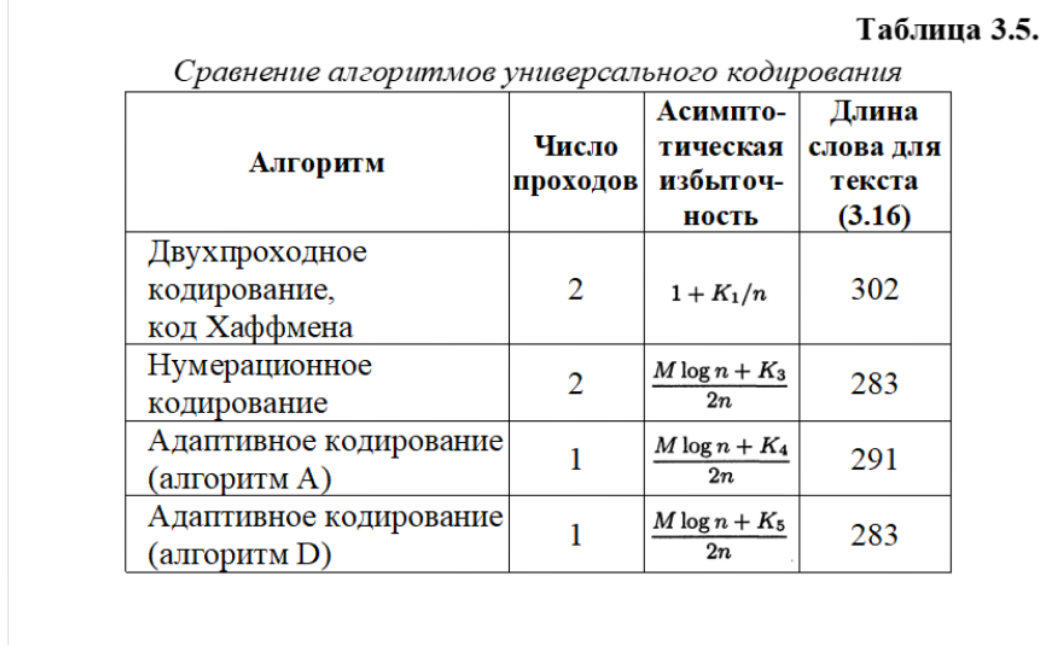
\includegraphics[width=90mm]{compare.png}
\caption{Сравнение способов кодирования}
\end{figure}

\bigskip
\textbf{62. Монотонные коды: унарный код, код Голомба, код Галлагера-Ван Byxpиca, код Левенштейна, код Элайеса.} \\

Унарный код. Запись вида \(0^m\) или \(1^m\) означает серию из \(m\) нулей или единиц соответственно. Унарный код сопоставляет числу \(i\) двоичную комбинацию вида \(1^{i-1}0\). Например, унарными кодами чисел 1, 2 и 3 являются последовательности \[unar(1)=0, unar(2)=10, unar(3)=110\]

Длина кодового слова для числа \(i\) равна \(l_i = i\).

Унарный код оптимален (минимизирует среднюю длину кодовых слов). если числа \(i\) распределены по геометрическому закону \[p_i = (1 - \alpha)\alpha^{i-1}, i = 1, 2...\] с параметром \(\alpha = 1/2\), то есть при \(p_i = 2^{-i}, i = 1, 2, ...\)

Для значений \(\alpha > 1/2\) более эффективен код Голомба. Код Голомба. Введем параметр \(T = 2^m\). Код Голомба для числа \(i\) состоит из двух частей. Первая часть - унарный код числа \(\lfloor i/T \rfloor + 1\), вторая — двоичная запись остатка от деления \(i\) на \(T\) в виде последовательности длины \(m\). Длина кода Голомба для числа \(i\) равна \(l_i = \lfloor i/T \rfloor + 1 + m\). Например, при \(m = 3\) и \(i = 21\) имеем \(\lfloor i/T \rfloor + 1 = 3\), остаток равен 5. Поэтому кодом Голомба числа 21 будет последовательность
\begin{displaymath}
    (110)(101)= 110101
\end{displaymath}
т.е.
\begin{displaymath}
    (unar(3))(bin(5))
\end{displaymath}

В технической литературе код Голомба иногда называют кодом Райса.

Код Галлагера-Ван Вухриса — естественное обобщение кода Голомба на случай, когда параметр \(T\) не является степенью двойки. Вычисляется префикс — это закодированное унарным кодом число \(\lfloor i/T \rfloor\). Далее следует двоичный код остатка.

Если \(\log T\) не целое число, то для представления некоторых (меньших) значений остатка от деления \(i\) на \(T\) используется \(m = \lfloor \log T \rfloor\) бит, а для остальных (больших) значений используется \(m + 1\) бит. Остаток кодируется кодом Хаффмена в предположении, что все значения остатка равновероятны. Например, при \(T\) = 5 кодовыми словами для значений остатков 0, 1, 2, З и 4 будут последовательности 00, 01, 10, 110 и 111 соответственно.

Оптимальное значение параметра \(T\) для кода Галлагера-Ван Вухриса связано с параметром геометрического распределения а соотношением
\begin{displaymath}
    \alpha^T + \alpha^{T+1} \leq \alpha^T + \alpha^{T-1}
\end{displaymath}

Благодаря чрезвычайно простой схеме кодирования и достаточно высокой эффективности коды Голомба и Галлагера-Ван Вухриса часто применяют при кодировании аудио- и видеосигналов.

Код Левенштейна. Предположим, что нужно передать число \(i = 21\). Двоичное представление этого числа имеет вид 10101. Непосредственно использовать при кодировании двоичные представления натуральных чисел нельзя, ибо такой код не будет префиксным. Самый простой выход состоит в том, чтобы приписать в начале слова префикс, указывающий длину двоичной записи числа (в данном случае это число 5). Если это число закодировать префиксным (например. унарным) кодом и приписать слева к двоичной записи числа, то код получится однозначно декодируемым. В данном примере для числа 21 получим кодовое слово \[[(unar(5))(bin(21))] \to (11110)(10101) = 1111010101\] В общем случае длина двоичного представления будет равна \(2 \lceil \log i\rceil\).

Пошагово улучшим способ кодирования - первая значашая цифра двоичной записи числа - всегда 1. Ее можно не передавать. декодер сам допишет недостающую единицу, если будет знать длину двоичной записи. Обозначим через \(bin'(i)\) двоичную запись натурального числа \(i\) без первой единицы, прямыми скобками обозначается длина двоичной последовательности.

Итак, простой монотонный код числа зимеет следующую структуру:
\begin{displaymath}
    mon(i) = (unar(|bin'(i)| + 1), bin'(i))
\end{displaymath}

Длины кодовых слов этого монотонного кода
\begin{displaymath}
    l_i = 2\lfloor \log i \rfloor + 1
\end{displaymath}

Чтобы сделать запись еще короче, с длиной двоичной записи можно поступить так же, как и с самим числом, то есть передать его значащие разряды (кроме первой единицы), затем длину двоичной записи числа значащих разрядов и т. д.

Итерации продолжаются, пока не останется один значащий разряд. Чтобы декодирование было однозначным, достаточно приписать префикс. содержащий закодированное префиксным кодом число итераций.

Минимальное число итераций равно 0 (при кодировании числа 1). Поэтому в качестве префиксного кода можно выбрать унарный код увеличенного на 1 числа итераций. Полученное кодовое слово будет кодовым словом кода Левенштейна.

Упрощенный код Левенитейна (код Элайеса). Более простой код приведен в работе Элайеса. Числу \(i = 1\) припишем кодовое слово \(elias(1) = 0\). Для чисел \(i > 1\) кодовые слова вычисляются по следующем правилу:
\begin{displaymath}
    elias(i)=(unar(|bin'(|bin'(i))|+2), bin'(|bin'(i)|), bin'(i))
\end{displaymath}

Кодовое слово состоит из 3 частей. Справа (в третьей части) записано двоичное представление числа без первой единицы. ей предшествует вторая часть, в которой пишется двоичное представление длины третьей части, тоже без первой единицы. Наконец, в первой части записан унарный код увеличенной на 2 длины второй части кодового слова.

Длина кодового слова кода Элайеса для произвольного числа \(i\)
\begin{displaymath}
    l_i = \left\{ \begin{array}{ll}
        1 & \textrm{\(i = 1\),}\\
        \lfloor \log i \rfloor + 2\lfloor \log \lfloor \log i \rfloor \rfloor + 2 & \textrm{\(i > 1\),}\\
  \end{array} \right.
\end{displaymath}

\bigskip
\textbf{63. Теорема о средней длине кодовых слов (теорема 4.1 с доказательством).} \\

\textbf{ТЕОРЕМА 4.1.} Пусть случайная величина \(i\) принимает значения из множества чисел натурального ряда и распределение вероятностей случайной величины удовлетворяет условию: \(p_i \leq p_j\), если \(i > j\). Тогда при использовании кода Элайеса средняя длина кодовых слов \(\bar{l}\) удовлетворяет неравенству
\begin{displaymath}
    \bar{l} \leq H(1 + o(H))
\end{displaymath}

где через \(H\) обозначена энтропия случайной величины \(i\), и \(o(H) \to 0\) при \(H \to \infty\).

\textbf{Доказательство.} Прежде всего, из упорядоченности вероятностей по убыванию и условия нормировки вероятностей вытекают неравенства
\begin{displaymath}
    p_i \leq \frac{1}{i}, i \leq \frac{1}{p_i}, i = 1, 2, ...
\end{displaymath}
\begin{displaymath}
    \bar{l} = \sum_{i=1}^{\infty} l_i p_i \leq \sum_{i=1}^{\infty} p_i(\log i + 2 \log \log i + 2) \leq \sum_{i=1}^{\infty} p_i \log \frac{1}{p_i} + 2\sum_{i=1}^{\infty} p_i \log \left(1 + \log\frac{1}{p_i}\right) + 2 \leq H + 2\log(1 + H) + 2
\end{displaymath}

Здесь первое неравенство основано на (4.5). второе использует (4.6). Последнее неравенство основано на выпуклости \(\cap\) функции \( \log x\). Из (4.1) следует утверждение теоремы.

\bigskip
\textbf{64. Интервальное кодирование.} \\

Интервальное кодирование.
Пусть \(X = \{0, 1,...,M - 1\}\) - алфавит источника и на выходе источника наблюдается последовательность \(x_1, x_2,....\) Алгоритм описывается рекуррентно.

Предположим, что начальная часть последовательности \(x_1^{n-1} = (x_1,...,x_{n-1})\) уже закодирована и передана и, следовательно, известна декодеру.

Вместо буквы \(x_n\), передается длина интервала (количество букв) между предыдущим и текущим появлением данной буквы т. е. кодер вычисляет и передает минимальное число \(r_n = r\) такое, что \(x_{n-r} = x_n\).

Исходная последовательность \(x_1, x_2,....\) преобразуется в последовательность чисел \(r_1, r_2,....\) Для завершения описания алгоритма нужно определить правило вычисления интервалов для тех букв, которые не встречались в последовательности \(x_1^{n-1}\). Проше всего условиться о том, что первой передаваемой букве предшествовали все буквы алфавита в заранее согласованном (для определенности, в алфавитном) порядке.

\bigskip
\textbf{65. Метод «стопка книг».} \\

Метод «стопка книг».

Этот метод известен под названиями «move-to-front coding» и «recency rank coding» («кодирование степени новизны»).

Как и при кодировании длин интервалов, предположим, что начальная часть последовательности \(x_1^{n-1} = (x_1,...,x_{n-1})\) уже закодирована и передана и, следовательно, известна декодеру.

Но теперь вместо буквы \(x_n\) передается количество различных букв  между предыдущим и текущим появлением данной буквы. Иными словами, кодер вычисляет минимальное число \(r_n = r\) такое, что \(x_{n-r} = x_n\).

Затем вычисляется число \(d_n\), различных букв в последовательности \(x_{n-r+1}^{n-1}\). Тем самым исходная последовательность \(x_1, x_2,....\) преобразуется в последовательность чисел \(d_1, d_2,....\) Для передачи букв, которые не встречались в \(x_1^{n-1}\), можно использовать стратегию для интервального кодирования.


\bigskip
\textbf{66. Теорема о средней скорости интервального кодирования (теорема 4.2 с доказательством).} \\

\textbf{ТЕОРЕМА 4.2.} Пусть \(H(X)\) — энтропия одномерного распределения дискретного стационарного источника. Средняя скорость интервального кодирования в сочетании с использованием кода Элайеса удовлетворяет неравенству
\begin{displaymath}
    \bar{R} \leq H(X)(1 + o(H(X)))
\end{displaymath}
где \(o(H) \to 0\) при \(H \to \infty\).

\textbf{Доказательство.} Обозначим через \(r_i(a)\) длину интервала между \(i\)-м и \(i-1\)-м появлениями буквы \(x = a\) и через \(l(a)\) соответствующие затраты на передачу буквы. В соответствии с оценкой (4.5)
\begin{displaymath}
    l_i(a) \leq \log r_i(a) + 2\log(1 + \log r_i(a)) + 2, (4.8)
\end{displaymath}

Обозначим через \(\bar{l}(a)\) и \(\bar{r}(a)\), соответственно, средние (по множеству последовательностей источника) затраты на передачу буквы \(a\) и среднюю длину интервала между появлениями буквы \(a\). В силу выпуклости логарифма из (4.8) после усреднения получаем
\begin{displaymath}
    \bar{l}(a) \leq \log \bar{r}(a) + 2\log(1 + \log \bar{r}(a)) + 2
\end{displaymath}

В соответствии с леммой Каца (Кас) (ее доказательство приведено ниже) имеет место неравенство
\begin{displaymath}
    \bar{r}(a) \leq \frac{1}{p(a)}
\end{displaymath}

Подставим эту оценку в (4.8) и усредним по всем буквам алфавита. Далее снова используем выпуклость логарифма. В результате получим
\begin{displaymath}
    \bar{R} = \sum_{a} p(a)\bar{l}(a) \leq H(X) + 2\log(1 + H(X)) + 2
\end{displaymath}

Преобразование потока данных с помошью интервального кодирования или кодирования по методу «стопки книг» с последующим применением кода Левенштейна (или кода Элайеса) гарантирует достаточно эффективное универсальное кодирование при простой реализации кодера и декодера.

\bigskip
\textbf{67. Лемма о случайной величине (лемма 4.3 с доказательством).} \\

\textbf{ЛЕММА 4.3.} Пусть случайная величина \(i\) принимает значения из множества натуральных чисел {1,2,...} в соответствии с распределением вероятностей \(\{p_i, i = 1,2,...\}\) Тогда
\begin{displaymath}
    M[i] = \sum_{i=1}^{\infty} P(i \geq j)
\end{displaymath}

\textbf{Доказательство.} \(P(i \geq j) = \sum_{i=1}^{\infty} p_i\). Сумма в правой части содержит
каждое слагаемое \(p_i\) ровно \(i\) раз. т.е. эта сумма равна математическому
ожиданию \(i\).

В теории вероятностей для дискретного случайного процесса \(x_0, x_1, ...\) длины интервалов между одинаковыми значениями процесса \(x_t = a\) называют временем возвращения процесса в состояние \(a\). Более точно, время возвращения в состояние \(a\) для стационарного процесса определяется как
\begin{displaymath}
    r = min\{k \geq 1: x_0 = x_k = a\}
\end{displaymath}

Распределение вероятностей времени возвращения в \(a\) определяется формулой
\begin{displaymath}
    q_a(r) = P(x_1,...,x_{r-q} \neq a, x_r = a | x_0 = a)
\end{displaymath}

соответственно, среднее время возвращения в \(a\)
\begin{displaymath}
    \bar{r}(a) = \sum_{r=1}^{\infty} r q_a(r)
\end{displaymath}

\bigskip
\textbf{68. Лемма Каца (лемма 4.4 с доказательством).} \\

\textbf{ЛЕММА 4.4.} (Лемма Каца) Для дискретного стационарного источника такого, что \(P(a) > 0\) справедливо соотношение \[\bar{r_a}p(a)= P(x_n = a \textrm{ хотя бы для одного } n, n = 0, 1, ...    (4.15)\]

В частности, для эргодического источника
\begin{displaymath}
    \bar{r}(a) \leq \frac{1}{p(a)}
\end{displaymath}

\textbf{Доказательство.} Рассмотрим произведение в левой части (4.15). Воспользовавшись леммой 4.3, получим
\begin{displaymath}
    \bar{r_a}p(a) = p(a) \sum_{t=1}^{\infty} r q_a(r) = p(a) \sum_{t=1}^{\infty} Q_a(t)
\end{displaymath}

где использовано обозначение
\begin{displaymath}
    Q_a(t) = \sum_{j=t}^{\infty} q_a(j) = P(r \geq t)
\end{displaymath}

Событие \(r \geq t\) (время возвращения в \(a\) не меньше \(t\)) имеет место в том случае, когда вслед за буквой \(a\) порождены \(t\) букв. ни одна из которых не совпадает с \(a\), то есть
\begin{displaymath}
    Q_a(t) = P(x_1,...,x_t \neq a|x_0 = a)
\end{displaymath}

Подстановка этого выражения дает
\begin{displaymath}
    \bar{r_a}p(a) = P(x_0 = a) \sum_{t=1}^{\infty} P(x_1,...,x_t \neq a|x_0 = a) = \sum_{t=1}^{\infty} P(x_0 = a,x_1,...,x_t \neq a)
\end{displaymath}

Введем распределение вероятностей на множестве последовательностей источника. Оно соответсвует инверсии во времени последовательностей исходного источника. обозначим его как  \(\tilde{p}(x), x \in X^n, n = 1, 2, ...\)

Для произвольного \(n\) и любой последовательности \(x = (x_1,...,x_n)\) обозначим через \(\overleftarrow{x}\) последовательность, полученную из \(x\)  инвертированием порядка следования символов, то есть \(\overleftarrow{x} = (x_n,...,x_1)\). По определению, \(\tilde{p}(\overleftarrow{x}) = p(x)\). Вероятности, вычисленные относительно этого распределения, будем обозначать как \(\tilde{p}(\cdot)\). Из последнего равенства с учетом стационарности инверсного процесса имеем
\begin{displaymath}
    \bar{r_a}p_a(t) = \sum_{t=1}^{\infty} \tilde{P}(x_0,...,x_{t-1} \neq a, x_t = a) = \tilde{P}(x_t = a \textrm{ хотя бы для одного } t, t = 1, 2, ...
\end{displaymath}

Вероятности появления хотя бы одной буквы \(a\) для исходного процесса и инверсного одинаковы. Для любого эргодического процесса и любой
буквы \(a\) такой, что \(p(a) > 0\) эта вероятность равна 1.

\bigskip
\textbf{69. Метод скользящего словаря (LZ-77): Алгоритм LZ-77, сложность алгоритма LZ-77, алгоритм LZFG.} \\

Данный алгоритм после его опубликования Зивом и Лемпелом в  был многократно модифицирован, некоторые модификации получили самостоятельные названия с аббревиатурами вида LZX, где X - первая буква имени автора модификации.

Рассмотрим формальное описание алгоритма.

Параметром алгоритма является длина «окна наблюдения» W. Эту величину можно также интерпретировать как «объем скользящего словаря».

Пусть \(X = \{0,1,..., M-1\}\) — алфавит источника и на выходе источника наблюдается последовательность \(х_1, х_2, ... ,х_n\). Алгоригм работы кодера показан на рис. 4.1.

\begin{figure}[ht!]
\centering
    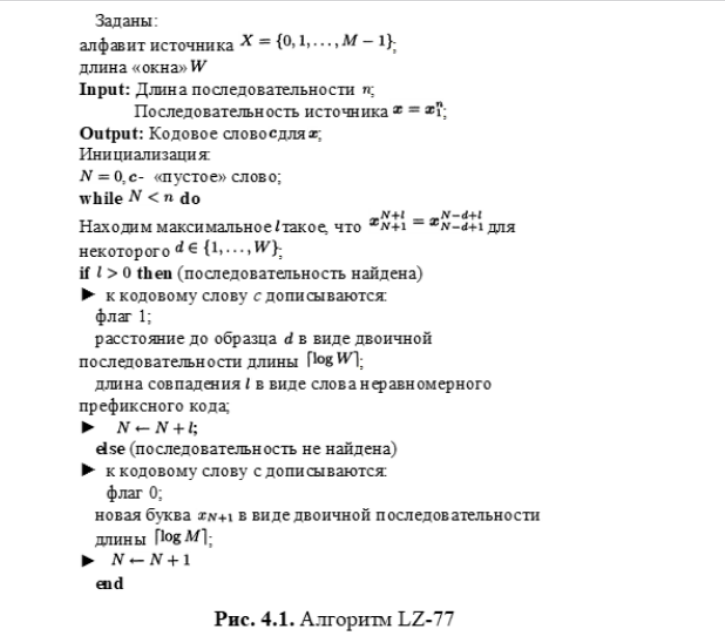
\includegraphics[width=90mm]{lz77_alg.png}
\caption{Алгоритм кодирования LZ-77}
\end{figure}


Кодер LZ-77 хранит в памяти скользящий словарь объемом W. Словами словаря служат всевозможные подпоследовательности следующих друг за другом букв. содержащиеся в последних W буквах источника.

При поступлении на вход кодера очередных букв источника кодер находит как можно более длинную последовательность, уже имеющуюся в словаре. В канал передается флаг (1 или 0). указывающий на то, найдено или нет подходящее словарное слово.

В случае успеха (флаг равен 1) словарное слово передается указанием удаления начала слова от текущей позиции и длины словарного слова.

Сложность алгоритма. Сложность кодирования и декодирования не равны. Вычислительная сложность декодирования очень низкая. Декодер непосредственно из битового потока получает информацию о том, начиная с какой буквы и какой длины последовательность букв он должен извлечь из памяти и выдать получателю.

Кодер для каждого из значений \(l = 1, 2...\) должен повторить попытку поиска в окне длиной W (типичные размеры окна составляют от 2048 до 16384 символов) образцов. совпадающих с вновь поступившими буквами источника. Такая «прямолинейная» реализация алгоритма неприемлемо сложна. Поэтому применяемые в архиваторах кодеры для быстрого поиска образцов в словаре кодера используют хеширование.

Вариант алгоритма LZFG (авторы Фиала и Гриине), приведенный на рис. 4.2.

\begin{figure}[h!]
\centering
    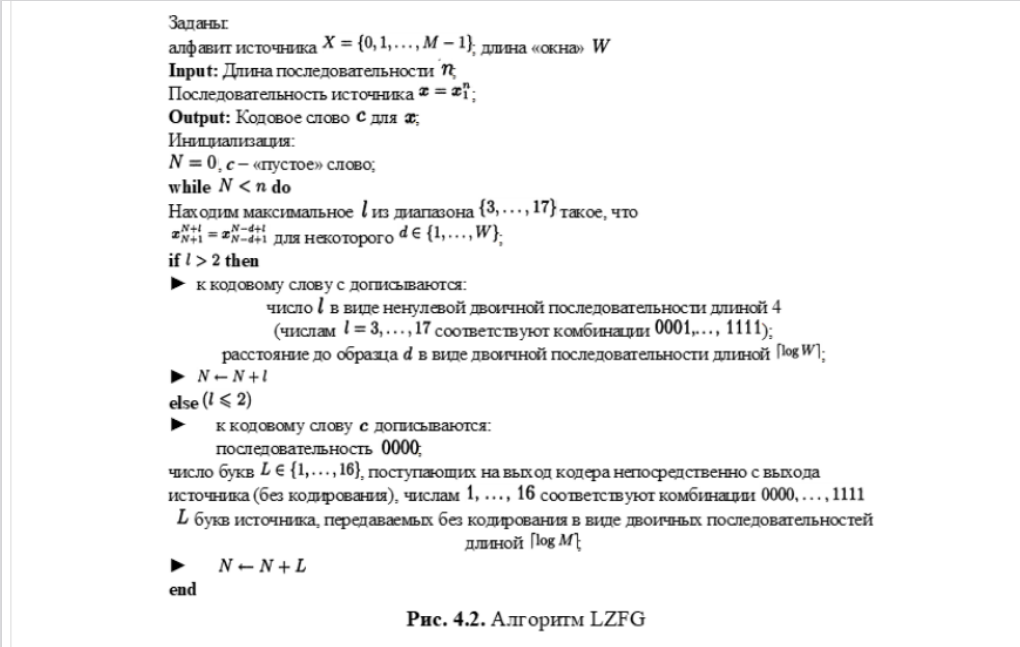
\includegraphics[width=90mm]{lzfg_alg.png}
\caption{Алгоритм кодирования LZFG}
\end{figure}

\bigskip
\textbf{70. Алгоритм LZW (LZ-78).} \\

Идея алгоритма состоит в том, что вместо последовательностей букв передаются номера слов в некотором словаре. Кодер и декодер в процессе работы синхронно формируют этот словарь. На каждом шаге словарь пополняется одним новым словом, которое до этого в словаре отсутствовало, но является продолжением на одну букву одного из слов словаря.

Пусть \(X = \{0,1,...,M-1\}\) — алфавит источника и на выходе источника наблюдается последовательность \(x_1, x_2, ...\) Для простоты описания алгоритма будем считать, что в начале работы кодера каждая из букв алфавита является словом длиной 1 и входит в состав словаря.

На каждом следующем шаге находим самое длинное слово, совпадающее с началом подлежащей кодированию последовательности. Пусть \(l\) — длина совпадения. Эти \(l\) букв передаются в виде ссылки на соответствующее слово словаря. Если объем словаря равен \(c\), то для передачи этой ссылки достаточно \(\lceil \log(c - 1) \rceil\) бит. Словарь пополняется новым словом, которое получается дописыванием к использованному на данном шаге слову следующей за ним в потоке кодируемых данных буквы.

Поскольку декодер не знает еще этой новой буквы, он сможет выполнить эту операцию только с задержкой на один шаг. Чтобы избежать неоднозначности кодирования, мы запрещаем кодеру пользоваться последним построенным словом словаря, что отражено в алгоритме на рис. 4.3. Исключение составляет первый шаг, когда словарь полностью известен кодеру и декодеру.

\begin{figure}[t!]
\centering
    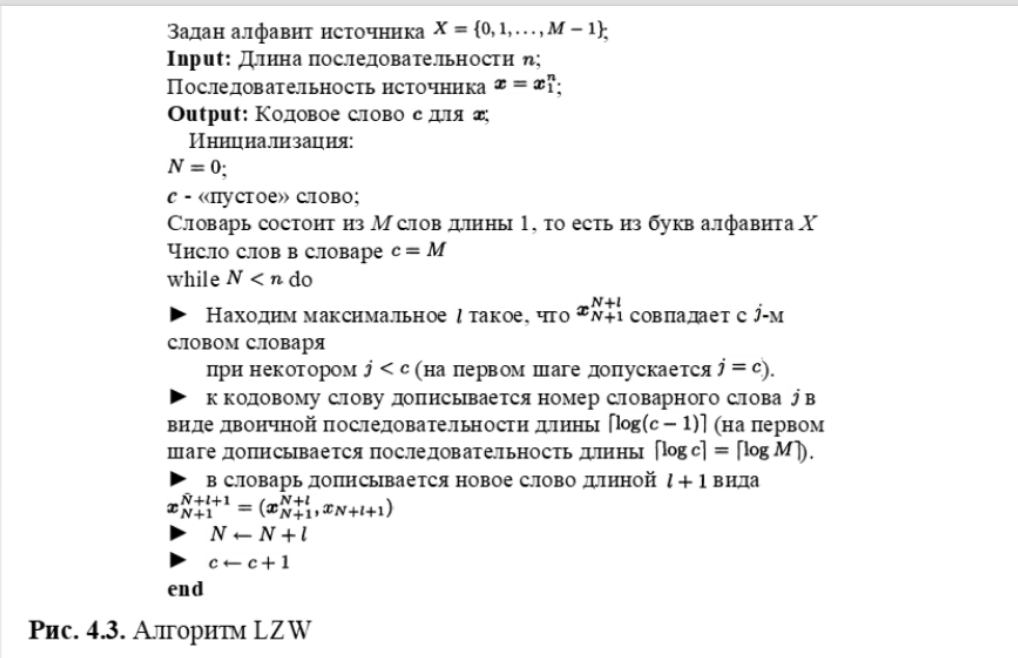
\includegraphics[width=90mm]{lzw_alg.png}
\caption{Алгоритм кодирования LZW}
\end{figure}

\bigskip
\textbf{71. Предсказание по частичному совпадению: идея алгоритма PPM.} \\

Рассмотрим наиболее «логичный» алгоритм кодирования при неизвестной статистике источника. На первый взгляд он является почти тривиальным развитием адаптивного арифметического кодирования.

Разница состоит в том, что в процессе кодирования вместо безусловных вероятностей букв оцениваются их условные вероятности, при известном «контексте», то есть при известных предшествующих буквах. Этот метод кодирования получил название РРМ (prediction by partian matching).

Предположим, что последовательность \(x_1^t = (x_1, ... , x_t)\) первых \(t\) букв источника уже передана и предстоит передать символ \(x_{t+1}\).

При кодировании очередной буквы выполняются следующие шаги.

1. Находим контекст \(x_{t-d+1}^{t}\) наибольшей длины \(d\). не превышающей заданной величины \(D\). Под контекстом — понимается последовательность \(s = x_{t-d+1}^{t}\), непосредственно предшествующая кодируемому символу и такая, что в точности такая же последовательность \(s\) уже встречалась в — переданной последовательности \(x_1^{t-1}\).

2. Для всех возможных значений символа \(x_{t+1}\) вычисляются оценки условных вероятностей символа при известном контексте \(s\).

3. Значение символа \(x_{t+1}\) кодируется арифметическим кодом в соответствии с вычисленной на шаге 2 оценкой условной вероятности.

Варианты алгоритма РРМ отличаются друг от друга выбором максимальной длины контекста \(D\) и, главное, способом выполнения шага 2. то есть вычисления оценки условной вероятности символа.

\begin{figure}[h!]
\centering
    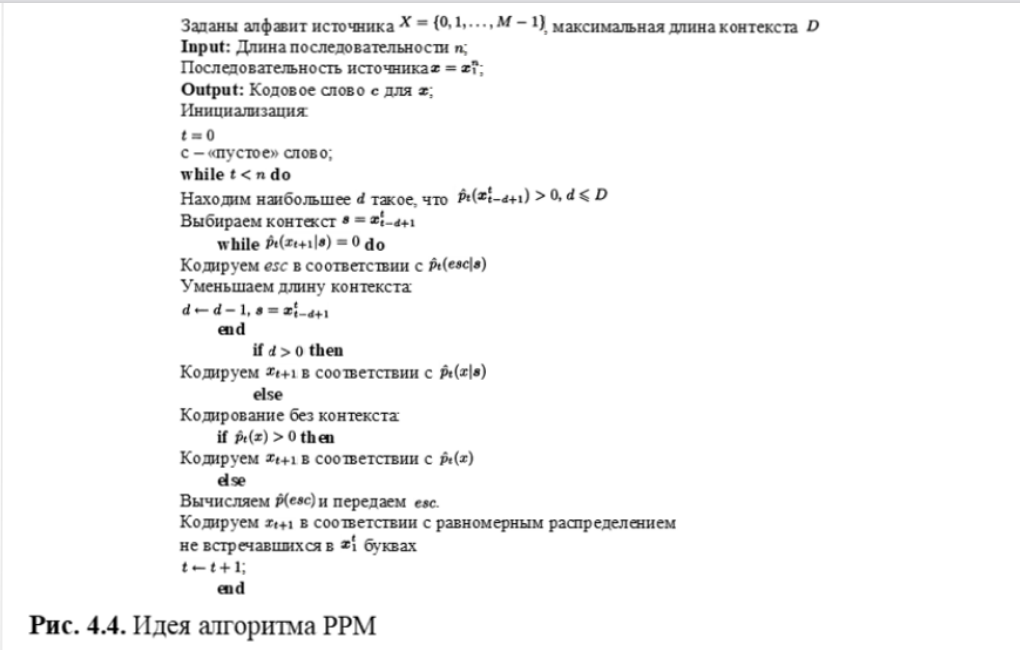
\includegraphics[width=90mm]{ppm_alg.png}
\caption{Алгоритм кодирования PPM}
\end{figure}

\bigskip
\textbf{72. Сжатие с использованием преобразования Барроуза-Уилера.} \\

Рассмотрим стационарный источник. Предположим, что модель источника может быть с достаточной точностью аппроксимирована цепью Маркова конечно связности \(m\).

При передаче длинной последовательности \(x = (x_1, ..., x_m\) подпоследовательность \(s = (s_1, ..., s_m\) встретится в тексте длиной \(n\) приблизительно \(np(s)\) раз. После циклического упорядочивания мы получим \(np(s)\) строк, которые будут начинаться с \(s = (s_1, ..., s_m\), распределение вероятностей букв в последнем столбце в этой части таблицы будет иметь вид \(p(x|s)\).

Использование одного из универсальных кодов, например, метода «стопки книг», позволит потратить на передачу этой части последовательности примерно \(np(s)H(X|s)\) бит. Суммируя по всем последовательностям \(s\). приходим к скорости кодирования близкой к \(H(X|X^m)\).

Выход преобразователя — это нестационарная последовательность, которая состоит из стационарных подпоследовательностей, соответствующих различным состояниям исходного источника.

Данный алгоритм хорошо подходит для источников, которые могут быть аппроксимированы моделью с относительно небольшим числом состояний, причем при известном состоянии условное распределение вероятностей должно быть близким к вырожденному (иметь небольшую энтропию). Этим условиям в большой степени удовлетворяют некоторые тексты, листинги программ и т. п.

\bigskip
\textbf{73. Сравнение способов кодирования, использующихся для сжатия.} \\

Сравним рассмотренные алгоритмы. Используем для сравнения текст из 50 букв, на котором мы иллюстрировали принципы работы алгоритмов. Результаты вычислений сведены в табл. 4.10. Хотя маленькая длина текста не позволяет делать надежных выводов о сравнительных характеристиках алгоритмов. тем не менее приведенные в таблице данные довольно — показательны.

Предложенные относительно недавно алгоритмы PPMD и кодирование с использованием преобразования Барроуза-Уилера существенно эффективнее других методов кодирования.

Однако при сравнении рассмотренных алгоритмов в реальных условиях применения можно увидеть. что однозначного решения эта задача не имеет. В частности, при кодировании различных файлов данных предпочтительными будут различные алгоритмы.

\begin{figure}[h!]
\centering
    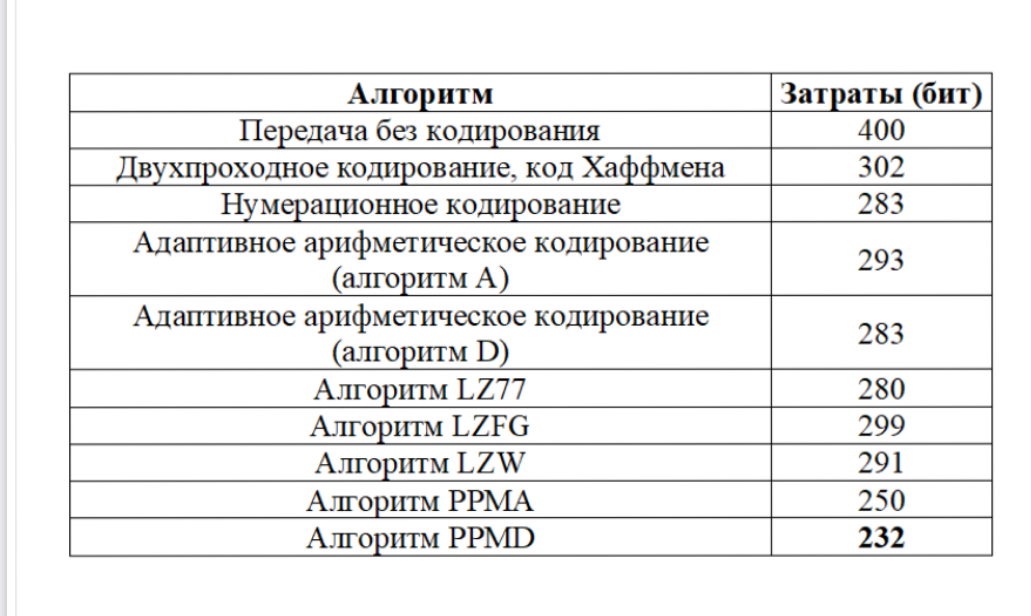
\includegraphics[width=90mm]{compare_archive_algs.png}
\caption{Сравнение алгоритмов для сжатия данных}
\end{figure}

\bigskip
\textbf{74. Скорость помехозащищенного кода. Пропускная способность канала.} \\

В качестве множества сообщений без потери общности можно
рассматривать множество чисел \(U = \{1,...,M\}\).

Кодом канала над алфавитом \(X\) называется любое множество последовательностей \(A = \{x_m\}, m = 1, ..., M, A \in X^n\). Сами последовательности называются кодовыми словами их длина \(n\) называется длиной кода, количество последовательностей \(M\) называется мощностью кода, величина
\begin{displaymath}
    R = \frac{\log M}{n}
\end{displaymath}
называется скоростью кода. 

Скорость кода измеряется в битах на символ канала. В частном случае, когда \(M = 2^k\), каждому из кодовых слов можно сопоставить последовательность из \(k\) информационных символов (\(k\) бит). Для их передачи будет использовано кодовое слово длиной \(n\).

Число \(C\) называется пропускной способностью канала, если при любой скорости кода \(R < C\) существуют коды, обеспечивающие сколь угодно малую вероятность ошибки и, напротив, при \(R > C\) существует константа \(\epsilon > 0\) такая, что вероятность ошибки любого кода ограничена снизу величиной \(\epsilon\) (то есть вероятность ошибки не может быть сделана сколь угодно малой).

\bigskip
\textbf{75. Модель канала. Канал без памяти. Двоичный симметричный канал (ДСК). Двоичный симметричный канал со стираниями (ДСтК).} \\

Модель канала задана, если для любых \(n\) и любых последовательностей \(x \in X^n\), \(x \in X^n\) указано правило вычисления условной вероятности \(p(y|x)\).

Обозначение \(x_i^n = (x_i, ..., x_n)\): канал называется стационарным, если для любых \(j\) и \(n\) и любых \(x_{j+1}^{j+n} \in X^n, y_{j+1}^{j+n} \in Y^n\) условные вероятности \(p(y_{j+1}^{j+n}|x_{j+1}^{j+n})\) определяются однозначно значениями символов последовательностей и не зависят от положения последовательностей во времени (от индекса \(j\)).

Канал называется каналом без памяти, если для любых \(j\) и \(n\) и любых \(x_{j+1}^{j+n} \in X^n, y_{j+1}^{j+n} \in Y^n\)
\begin{displaymath}
    p(y_{j+1}^{j+n}|x_{j+1}^{j+n}) = \prod_{i=j+1}^{j+n} p(y_i|x_i)
\end{displaymath}

Согласно данному определению, в канале без памяти события, происходящие при передаче последовательных символов, независимы.

Стационарный канал без памяти называют дискретным постоянным каналом (ДПК).

Классификация каналов аналогична классификации источников. Однако задача кодирования для каналов значительно сложнее.

Для описания ДПК достаточно указать одномерные условные вероятности \(\{p(y|x), x \in X, y \in Y\}\).

Положим \(X = \{0,...,K - 1\}, Y = \{0,...,L - 1\}\). Обозначим \(p_{ij} = p(y = j|x = i), i \in X. j \in Y\) Переходные вероятности канала \(p_{ij}\) удобно записывать в виде матрицы
\begin{displaymath}
 \begin{pmatrix}
     p_{0,0} & p_{0,1} & \cdots & p_{0,L-1} \\
     p_{1,0} & p_{1,1} & \cdots & p_{1,L-1} \\
  \vdots  & \vdots  & \ddots & \vdots  \\
  p_{K-1,0} & p_{K-1,1} & \cdots & p_{K-1,L-1} \\
 \end{pmatrix}
\end{displaymath}

Эта стохастическая матрица называется матрицей переходных вероятностей канала. Она полностью описывает модель ДПК. Приведем два простых. но важных примера ДПК.

Пример 5.2.1. Двоичный симметричный канал (ДСК). Для данной модели \(X = Y = \{0,1\}\), а переходные вероятности удовлетворяют условиям \(p_{10} = p_{01} = p, p_{00} = p_{11} = 1 - p\) Матрица переходных вероятностей имеет вид
\begin{displaymath}
    P = 
 \begin{pmatrix}
     1 - p & p \\
     p & 1 - p \\
 \end{pmatrix}
\end{displaymath}

Пример 5.2.2. Двоичный симметричный канал со стираниями (ДСтК). Матрица переходных вероятностей имеет вид
\begin{displaymath}
    P = 
 \begin{pmatrix}
     1 - p - \epsilon & \epsilon & p \\
     p & \epsilon & 1 - p - \epsilon \\
 \end{pmatrix}
\end{displaymath}

Входной алфавит ДСтК содержит два символа, 0 и 1, а выходной алфавит помимо этих двух символов содержит дополнительный символ \(\epsilon\), который называют символом стирания.

В ДСтК каждый из входных символов может с вероятностью \(p\) превратиться в противоположный символ и с вероятностью \(\epsilon\) может принять неопределенное значение, называемое стиранием.

Вероятности ошибки \(p\) стирания \(\epsilon\) постоянны, они не зависят от результатов передачи предыдущих и следующих символов и от
значения передаваемого в данный момент символа.

\bigskip
\textbf{76. Дискретный постоянный канал. Матрица переходных вероятностей канала.} \\

Канал называется каналом без памяти, если для любых \(j\) и \(n\) и любых \(x_{j+1}^{j+n} \in X^n, y_{j+1}^{j+n} \in Y^n\)
\begin{displaymath}
    p(y_{j+1}^{j+n}|x_{j+1}^{j+n}) = \prod_{i=j+1}^{j+n} p(y_i|x_i)
\end{displaymath}

Согласно данному определению, в канале без памяти события, происходящие при передаче последовательных символов, независимы.

Стационарный канал без памяти называют дискретным постоянным каналом (ДПК).

Классификация каналов аналогична классификации источников. Однако задача кодирования для каналов значительно сложнее.

Для описания ДПК достаточно указать одномерные условные вероятности \(\{p(y|x), x \in X, y \in Y\}\).

Положим \(X = \{0,...,K - 1\}, Y = \{0,...,L - 1\}\). Обозначим \(p_{ij} = p(y = j|x = i), i \in X. j \in Y\) Переходные вероятности канала \(p_{ij}\) удобно записывать в виде матрицы
\begin{displaymath}
 \begin{pmatrix}
     p_{0,0} & p_{0,1} & \cdots & p_{0,L-1} \\
     p_{1,0} & p_{1,1} & \cdots & p_{1,L-1} \\
  \vdots  & \vdots  & \ddots & \vdots  \\
  p_{K-1,0} & p_{K-1,1} & \cdots & p_{K-1,L-1} \\
 \end{pmatrix}
\end{displaymath}

Эта стохастическая матрица называется матрицей переходных вероятностей канала. Она полностью описывает модель ДПК.

\bigskip
\textbf{77. Взаимная информация канала. Средняя взаимная информация канала. Свойства взаимной информации.} \\

В каналах связи важным является возможность получения информации о передаваемых сообщениях по символам, наблюдаемым на входе канала. Говоря более формально, для заданного произведения \(XY = \{(x, y), p(x, y)\}\) дискретных ансамблей \(X\) и \(Y\) нужно количественно измерить информацию об элементах \(x \in X\) входного ансамбля, содержащуюся в выходных символах \(y \in Y\).

Подходящей мерой такой информации является взаимная информация, определяемая для любых пар \((x,y) \in XY\) соотношением \[ I(x;y) = I(x) - I(x|y) \]

В выражении \(I(x;y)\) в качестве разделителя используется точка с запятой, чтобы не перепутать эту величину с собственной информацией \(I(x,y)\) пары сообщений \((x,y)\).

Взаимная информация определена только для пар \((x,y)\), имеющих ненулевую вероятность.

Свойства взаимной информации:
\begin{itemize}
    \item Свойство 5.3.1. Симметричность: \(I(x;y) = I(y;x)\)
    \item Свойство 5.3.2. Если \(x\) и \(y\) независимы, то \(I(x;y) = 0\)
\end{itemize}

Средней взаимной информацией между ансамблями \(X\) и \(Y\) называется величина \[ I(X;Y) = \textbf{M}[I(x;y)] \]
Свойства средней взаимной информации:
\begin{itemize}
    \item Свойство 5.3.3. Симметричность: \(I(X;Y) = I(Y;X)\)
    \item Свойство 5.3.4. Неотрицательность: \(I(X;Y) \geq 0\)
    \item Свойство 5.3.5. Тождество \(I(X;Y) = 0\) имеет место тогда и только тогда, когда ансамбли \(X\) и \(Y\) независимы.
    \item Свойство 5.3.6. \(I(X;Y)= Н(X) - H(X|Y) = H(Y)— H(Y|X) = H(X) + H(Y) - H(XY)\)
    \item Свойство 5.3.7. \(I(X;Y) \leq \min\{H(X), H(X)\}\)
    \item Свойство 5.3.8. \(I(X;Y) \leq \min\{\log|X|, \log|Y|\}\)
    \item Свойство 5.3.9. Взаимная информация \(I(X;Y)\) - выпуклая \(\cap\) функция распределения вероятностей \(p(x)\)
    \item Свойство 5.3.10. Взаимная информация \(I(X;Y)\) - выпуклая \(\cup\) функция условных распределений \(p(y|x)\)
\end{itemize}

\bigskip
\textbf{78. Условная средняя взаимная информация. Теорема о переработке информации.} \\

Средней условной взаимной информацией между \(X\) и \(X\) при условии
\(Z\) называется величина
\begin{displaymath}
    I(X;Y|Z) = \textbf{M}[I(X;Y|z)] = \sum_{x \in X}\sum_{y \in Y}\sum_{z \in Z} p(x, y, z) \log\frac{p(y|x, z)}{p(y|z)}
\end{displaymath}

Разумеется, средняя условная информация обладает всеми свойствами средней взаимной информации.

Система обработки информации.

Входом системы являются элементы ансамбля \(X\), выход первого
устройства \(Y\) является входом второго, а выход второго устройства \(Z\)
является выходом всей системы. Специфической особенностью
распределения вероятностей на множестве \(XYZ\) является условная
независимость \(X\) и \(Z\) при известном \(Y\). Следствием этой
независимости является теорема, называемая теоремой о переработке
информации.

\textbf{ТЕОРЕМА 5.1.} Пусть \(X\), \(Y\) и \(Z\) - вероятностные ансамбли, формируемые системой последовательной обработки информации. Тогда имеют место неравенства:
\begin{displaymath}
    I(X;Y) \geq I(X;Z)
\end{displaymath}
\begin{displaymath}
    I(Y;Z) \geq I(X;Z)
\end{displaymath}

\bigskip
\textbf{79. Информационная емкость канала.} \\

Величина 
\begin{displaymath}
    C_0 = \sup_{n}\max_{\{p(x)\}}\frac{1}{n} I(X^n;Y^n)
\end{displaymath}
называется информационной емкостью канала.

Пусть, например. \(A = \{(n - 1)/n, n = 1, 2,...\}\). Максимального числа
в этом множестве не существует, но \(\sup A = 1\), причем эта верхняя грань
совпадает с пределом последовательности при \(n \to \infty\).

Аналогично в определении информационной емкости канала
наибольшее значение средней взаимной информации на букву канала
может достигаться при бесконечной длине кода, поэтому в формуле 
используется именно верхняя грань, а не максимальное значение.

Информационную емкость канала \(C_0\) определим как некоторую
функцию его переходных вероятностей. Мы предполагаем, что именно
эта величина характеризует потенциально достижимую скорость
передачи по каналу.

\bigskip
\textbf{80. Неравенство Фано (с доказательством)} \\

\textbf{ТЕОРЕМА 5.2.} (Неравенство Фано)
\begin{displaymath}
    H(U|V) \leq \eta(P_e) + P_e\log(M - 1), (5.15)
\end{displaymath}
где \(\eta(\cdot)\) обозначает энтропию двоичного ансамбля.

\textbf{Доказательство.} Используя (5.13) и (5.14). запишем выражения,
участвующие в неравенстве Фано (5.15), в следующем виде:
\begin{displaymath}
    H(U|V) = -\sum_{u}\sum_{\upsilon \neq u} p(u, \upsilon) \log p(u|\upsilon) - \sum_{u}\sum_{\upsilon = u} p(u, \upsilon) \log p(u|\upsilon), (5.17)
\end{displaymath}
\begin{displaymath}
    \eta(P_e) = -\sum_{u}\sum_{\upsilon \neq u} p(u, \upsilon) \log P_e - \sum_{u}\sum_{\upsilon \neq u} p(u, \upsilon) \log P_c, (5.18)
\end{displaymath}
\begin{displaymath}
    P_e \log(M - 1) = \sum_{u}\sum_{\upsilon \neq u} p(u, \upsilon) \log (M - 1), (5.19)
\end{displaymath}


Рассмотрим разность
\begin{displaymath}
    \Delta = H(U|V) - \eta(P_e) - P_e \log(M - 1)
\end{displaymath}

Чтобы доказать (5.15). нужно доказать, что \(\Delta \leq 0\). Для этого вычтем
из правой и левой части (5.17) соответствующие части тождеств (5.18)
и (5.19). После элементарных преобразований придем к равенству
\begin{displaymath}
    \Delta = \sum_{u}\sum_{\upsilon \neq u} p(u, \upsilon) \log \frac{P_e}{p(u|\upsilon)(M - 1)} + \sum_{u}\sum_{\upsilon = u} p(u, \upsilon) \log\frac{P_c}{p(u|\upsilon)}
\end{displaymath}

Следующий шаг основан на использовании неравенства \(\log X \leq (x - 1)\log e\).

Применив его к обоим слагаемым, получим

\begin{displaymath}
    \begin{aligned}
        \Delta \leq(\log e) & \left[ \sum_{u}\sum_{\upsilon \neq u} p(u, \upsilon) \log \frac{P_e}{p(u|\upsilon)(M - 1)} - \sum_{u}\sum_{\upsilon \neq u} p(u, \upsilon) + \sum_{u}\sum_{\upsilon = u} p(u, \upsilon) \log\frac{P_c}{p(u|\upsilon)} - \sum_{u}\sum_{\upsilon = u} p(u, \upsilon) \right]
    \end{aligned}
\end{displaymath}

Воспользуемся тем, что \(p(u, \upsilon) = p(\upsilon)p(u|\upsilon)\). и обозначениями (5.13) и (5.14).

Результат легко привести к виду
\begin{displaymath}
    \Delta \leq (\log e) \times \left[ \frac{P_e}{M - 1}\sum_{u}\sum_{\upsilon \neq u} p(\upsilon)  - P_e + P_c \sum_{u}\sum_{\upsilon = u} p(\upsilon) - P_c \right], (5.20)
\end{displaymath}

Заметим теперь, что
\begin{displaymath}
    \sum_{u}\sum_{\upsilon \neq u} p(\upsilon) = (M - 1) \sum_{\upsilon} p(\upsilon) = M - 1, (5.21)
\end{displaymath}

Сумма в левой части содержит всего \(M\) различных слагаемых, и
каждое из них встречается в этой сумме ровно \((M - 1)\) раз. Кроме того,
справедливо равенство
\begin{displaymath}
    \sum_{u}\sum_{\upsilon = u} p(\upsilon) = \sum_{\upsilon} p(\upsilon) = 1, (5.22)
\end{displaymath}

Подстановка (5.21) и (5.22) в (5.20) приводит к неравенству \(\Delta \leq 0\).
Тем самым неравенство Фано доказано.

\bigskip
\textbf{81. Теорема для последовательностей, составленных из элементов множества объема М (теорема 5.3)} \\

\textbf{ТЕОРЕМА 5.3.} Для последовательностей \((u, \upsilon) \in U^N V^N\),
составленных из элементов множества объема \(M\). имеет место
неравенство
\begin{displaymath}
    \frac{1}{N}H(U^N|V^N) \leq \eta(\bar{P_e}) + \bar{P_e}\log(M - 1)
\end{displaymath}

\textbf{Доказательство.} Напомним, что условная энтропия не возрастает с увеличением числа условий. Поэтому
\begin{displaymath}
    H(U^N|V^N) = \sum_{i=1}^{N} H(U_i|U_1...U_{i-1}V^N) \leq \sum_{i=1}^{N} H(U_i|V_i)
\end{displaymath}

Поделим обе части на \(N\) и к каждому слагаемому применим
неравенство Фано. Получим
\begin{displaymath}
    \frac{1}{N}H(U^N|V^N) \leq \frac{1}{N}\sum_{i=1}^{N} \eta(P_{ei}) + \frac{1}{N}\sum_{i=1}^{N} P_{ei}\log(M - 1)
\end{displaymath}

Поскольку энтропия - выпуклая \(\cap\) функция, средняя по \(i\) энтропия
не меньше энтропии средней вероятности ошибки. Учитывая это, из
последнего неравенства получаем доказываемое неравенство.

\bigskip
\textbf{82. Обратная теорема кодирования.} \\

\textbf{ТЕОРЕМА 5.4.} Обратная теорема кодирования. Для дискретного
стационарного канала с информационной емкостью \(C_0\) для любого
\(\delta > 0\) существует число \(\epsilon > 0\), такое, что для любого кода со
скоростью \(R > C_0 + \delta\) средняя вероятность ошибки удовлетворяет
неравенству \(P_e \geq \epsilon\).

\textbf{Доказательство.} Рассмотрим произвольный код \(C\) длиной \(n\) со
скоростью \(R = \log|C|/n\). Обозначим через \(N\) длину последовательностей
сообщений \(u \in U^N\), сопоставляемых словам кода \(C\), через \(\upsilon \in V^N\)
обозначим последовательности решений, принимаемых декодером.
Имеет место цепочка соотношений
\begin{displaymath}
    \begin{aligned}
        nR = \log|C| = H(X^n) & \leq H(U^N) = H(U^N) - H(U^n|V^N) + H(U^N|V^N) = I(U^N;V^N) + H(U^N|V^N) \leq \\
        & \leq I(X^n;Y^n) + H(U^N|V^N) \leq nC_0 + n\gamma(\bar{P_e}) \\
    \end{aligned}
\end{displaymath}

Из последнего неравенства получаем
\begin{displaymath}
    \gamma(\bar{P_e}) \geq R - C_0 > \delta
\end{displaymath}

Из свойств функции \(\gamma(\cdot)\) следует, что из неравенства \(\gamma(\bar{P_e}) > \delta\)
следует существование положительного \(\epsilon > 0\) такого, что \(P_e \geq \epsilon\).
Теорема доказана.

\bigskip
\textbf{83. Вычисление информационной емкости каналов без памяти (теорема с доказательством).} \\

\textbf{ТЕОРЕМА 5.5.} Информационная емкость дискретного
постоянного канала вычисляется по формуле
\begin{displaymath}
    C_0 = \max_{\{p(x)\}} I(X;Y), (5.26)
\end{displaymath}

\textbf{Доказательство.} Доказательство состоит из двух шагов. Сначала
докажем, что правая часть (5.26) является границей сверху на
информационную емкость канала. Затем докажем, что эта граница
достигается при некотором распределении \(p(x)\).

При произвольном распределении \(\{p(x), x \in X^n\}\) запишем взаимную
информацию между входными и выходными последовательностями в
виде
\begin{displaymath}
    I(X^n;Y^n) = H(Y^n) - H(Y^n|X^n), (5.27)
\end{displaymath}

Воспользовавшись (5.24) и свойствами логарифма и
математического ожидания, выполним простые преобразования.
\begin{displaymath}
    \begin{aligned}
    H(Y^n|X^n) = \textbf{M}[-\log p(y|x)] = \textbf{M} \left[-\log \prod_{i=1}^{n} p(y_i|x_i) \right] = \\
        = \sum_{i=1}^{n} \textbf{M}[-\log p(y_i|x_i)] = \sum_{i=1}^{n} H(Y_i|X_i)
    \end{aligned}
\end{displaymath}

Из свойств энтропии
\begin{displaymath}
    H(Y^n) \leq \sum_{i=1}^{n} H(Y_i), (5.28)
\end{displaymath}

причем равенство имеет место только для независимых ансамблей.
С учетом выполненных выкладок вместо (5.27) получаем неравенство
\begin{displaymath}
    I(X^n;Y^n) \leq \sum_{i=1}^{n}[H(Y_i) - H(Y_i|X_i)] = \sum_{i=1}^{n} I(X_i;Y_i), (5.29)
\end{displaymath}

Завершили первый шаг доказательства. Предположим теперь, что
буквы на входе канала независимы, и докажем, что при этом
предположении в (5.29) имеет место равенство. Это будет означать.
что максимум в (5.25) следует искать только среди таких
распределений на \(X^n\), которые порождают последовательности
независимых букв на выходе канала.

Доказательство сводится к доказательству того, что при этом
предположении имеет место равенство в (5.28). То есть, нужно
доказать, что для дискретного канала без памяти из независимости
букв на входе канала следует независимость символов на выходе
канала.

Выходное распределение по формуле полной вероятности
вычисляется как
\begin{displaymath}
    p(y) = \sum_{x \in X^n} p(x)p(y|x)
\end{displaymath}

В предположении о независимости входных символов с учетом
(5.24) получаем
\begin{displaymath}
    \begin{aligned}
    p(y) = \sum_{x \in X^n} \prod_{i=1}^{n} p(x_i) \prod_{i=1}^{n} p(y_i|x_i) = \sum_{x \in X^n} \prod_{i=1}^{n} p(x_i)p(y_i|x_i) = \\
        = \sum_{x_1 \in X^n} \sum_{x_2 \in X^n} \ldots \sum_{x_n \in X^n} p(x_1)p(y_1|x_1) \cdot p(x_2)p(y_2|x_2) \cdot \ldots \cdot p(x_n)p(y_n|x_n) \\
    \end{aligned}
\end{displaymath}

Поочередно вынося сомнножители за знаки сумм, приходим к 
равенству
\begin{displaymath}
    p(y) =  \prod_{i=1}^{n} \sum_{x_i \in X^n} p(x_i)p(y_i|x_i) = \prod_{i=1}^{n} p(y_i)
\end{displaymath}
из которого и вытекает доказываемое утверждение о независимости
выходных символов канала.

\bigskip
\textbf{84. Симметричные каналы. Свойства симметричных каналов.} \\

ДПК называется симметричным по входу, если все строки его
матрицы переходных вероятностей могут быть получены
перестановками элементов первой строки.

ДПК называется симметричным по выходу, если все столбцы его
матрицы переходных вероятностей могут быть получены
перестановками элементов первого столбца.

ДПК называется полностью симметричным, если он симметричен
одновременно по входу и по выходу.

\begin{figure}[ht!]
\centering
    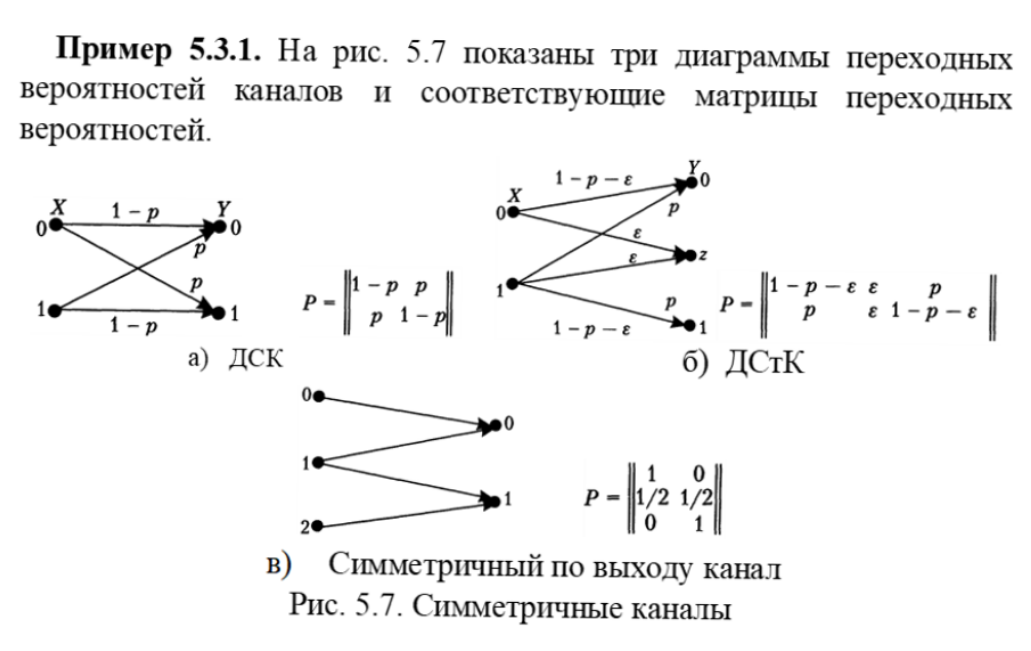
\includegraphics[width=90mm]{gates.png}
\caption{Симметричные каналы}
\end{figure}

Сформулируем те свойства симметричных каналов:
\begin{itemize}
    \item Свойство 5.4.1. Для симметричного по входу канала без памяти \(x \in X\) \[C_0 = \max_{\{p(x)\}} \{H(Y)\} - H(Y|x)\]
    \item Свойство 5.4.2. Для симметричного по входу канала без памяти \(x \in X\) \[C_0 \leq \log L -  H(Y|x)\]
    \item Свойство 5.4.3. Для симметричного по выходу канала без памяти при равновероятных входных символах выходные символы также равновероятны.
    \item Свойство 5.4.4. Для симметричного по входу канала без памяти \(x \in X\) \[C_0 = \log|Y| -  H(Y|x)\]
\end{itemize}

\bigskip
\textbf{85. Прямая теорема кодирования для дискретных постоянных каналов (теорема).} \\

\textbf{ТЕОРЕМА 5.6.} Для дискретного постоянного канала с
информационной емкостью \(C_0\) для любых \(\epsilon, \delta > 0\) существует
достаточно большое число \(n_0\) такое, что для любого натурального
числа \(n \geq n_0\) существует код длиной \(n\) со скоростью \(R \geq C_0 - \delta\), средняя
вероятность ошибки которого \(P_e < \epsilon\).

Иными словами, при скорости кода сколь угодно близкой к
информационной емкости \(C_0\) (но, конечно, меньшей \(C_0\) хотя бы на
малую величину \(\delta\)) увеличением длины кодовых слов можно добиться
сколь угодно малой вероятности ошибки (меньше любого \(\epsilon\))

Оптимистический результат, обещаемый случайным кодированием,
неконструктивен. Случайное кодирование - мощный метод анализа.
придуманный Шенноном, - не может быть использовано для
построения хороших кодов.

Для надежной передачи информации нужны довольно длинные
коды. С ростом длины кодов экспоненциально растет число кодовых
слов, а значит, и сложность описания кодов, сложность процедур
кодирования и декодирования.

Поэтому используемые на практике коды имеют регулярную
структуру, что делает возможной реализацию кодирования и
декодирования с разумной сложностью.
\end{document}
